
\documentclass[utf-8,8pt]{beamer}

\usepackage{amsmath,amssymb,amsfonts}
\usepackage{mathrsfs}
\usepackage{color,xcolor}
\usepackage{graphicx}
\usepackage{clock} % Use this package to insert a clock in the beamer.
\usepackage{textcomp}
\usepackage[T1]{fontenc}
\usepackage{epstopdf}
\mode<presentation>
{
  \usetheme{Warsaw}
  % 
  \setbeamercovered{transparent}
  %
}
% beamer
\usefonttheme{professionalfonts}
%\usepackage{CJK}
\usepackage{color}
\usepackage{xcolor}


\newcommand{\R}{\mathbb{R}}
%\newcommand{\C}{\mathbb{C}}
\renewcommand{\i}{\mathbf{i}}
\newcommand{\ii}{\mathbf{i}}
\renewcommand{\Re}{\mathrm{Re}\,}
\renewcommand{\Im}{\mathrm{Im}\,}
\newtheorem{algorithm}{Algorithm}[section]
\newtheorem{lem}{Lemma}[section]
\newtheorem{them}{Theorem}[section]
\newtheorem{assumption}{Assumption}[section]
\newtheorem{remark}{}[section]
%\newtheorem{definition}{Definition}[section]
\newtheorem{question}{}[section]
%\newtheorem{example}{\bf }[section]

\newcommand{\eps}{\varepsilon}
\newcommand{\RR}{\mathcal{R}}




\newcounter{RomanNumber}
\newcommand{\MyRoman}[1]{\rm\setcounter{RomanNumber}{#1}\Roman{RomanNumber}}

\newcommand{\bL}{\mathbf{L}}
\newcommand{\bH}{\mathbf{H}}
\newcommand{\bW}{\mathbf{W}}
\newcommand{\bP}{\mathbf{P}}
\newcommand{\bQ}{\mathbf{Q}}
\newcommand{\bp}{\mathbf{p}}
\newcommand{\bq}{\mathbf{q}}
\newcommand{\uL}{u_{_{\rm L}}}
\newcommand{\vL}{v_{_{\rm L}}}
\newcommand{\tuL}{\tilde u_{_{\rm L}}}
\newcommand{\tvL}{\tilde v_{_{\rm L}}}
\newcommand{\fL}{f_{_{\rm L}}}
\newcommand{\gL}{g_{_{\rm L}}}
\newcommand{\bpL}{\bp_{_{\rm L}}}
\newcommand{\bqL}{\bq_{_{\rm L}}}
\newcommand{\tbpL}{\tilde{\bp}_{_{\rm L}}}
\newcommand{\tbqL}{\tilde{\bq}_{_{\rm L}}}
\newcommand{\tbpLf}{\tilde{\bp}_{_{\rm L,1}}}
\newcommand{\tbpLs}{\tilde{\bp}_{_{\rm L,2}}}
\newcommand{\tbqLf}{\tilde{\bq}_{_{\rm L,1}}}
\newcommand{\tbqLs}{\tilde{\bq}_{_{\rm L,2}}}
\newcommand{\bn}{\nu}
\newcommand{\bv}{\mathbf{v}}
\newcommand{\om}{\omega}
\newcommand{\pa}{\partial}
\newcommand{\la}{\langle}
\newcommand{\ra}{\rangle}
\newcommand{\lla}{\la{\hskip -2pt}\la}
\newcommand{\rra}{\ra{\hskip -2pt}\ra}
\newcommand{\jj}{\|{\hskip -0.8pt} |}
\newcommand{\al}{\alpha}
\newcommand{\ze}{\zeta}
\newcommand{\si}{\sigma}
\newcommand{\ep}{\varepsilon}
\newcommand{\na}{\nabla}
\newcommand{\vp}{\varphi}
\newcommand{\ga}{\gamma}
\newcommand{\Ga}{\Gamma}
\newcommand{\Om}{\Omega}
\newcommand{\de}{\delta}
\newcommand{\Th}{\Theta}
\newcommand{\De}{\Delta}
\newcommand{\Lam}{\Lambda}
\newcommand{\lam}{\lambda}
\newcommand{\tri}{\triangle}
\newcommand{\lj}{[{\hskip -2pt} [}
\newcommand{\rj}{]{\hskip -2pt} ]}
\newcommand{\bks}{\backslash}
%\newcommand{\diag}{\mathrm{diag}}
\newcommand{\diam}{\mathrm{diam}}
\newcommand{\osc}{\mathrm{osc}}
\newcommand{\meas}{\mathrm{meas}}
\newcommand{\dist}{\mathrm{dist}}

\newcommand{\mL}{\mathscr{L}}
\newcommand{\cT}{{\cal T}}
\newcommand{\cM}{{\cal M}}
\newcommand{\cE}{{\cal E}}
\newcommand{\cL}{{\cal L}}
\newcommand{\cF}{{\cal F}}
\newcommand{\cB}{{\cal B}}
\newcommand{\PML}{{\rm PML}}
\newcommand{\FEM}{{\rm FEM}}
\newcommand{\rd}{\,\mathrm{d}}

\renewcommand{\i}{\mathbf{i}}
\renewcommand{\v}{\mathbf{v}}
\renewcommand{\u}{\mathbf{u}}
\renewcommand{\r}{\mathbf{r}}
\newcommand{\gR}{{\mathbb{R}}}
\newcommand{\Z}{{\mathbb{Z}}}
\renewcommand{\C}{{\mathbb{C}}}

\renewcommand{\Re}{\mathrm{Re}\,}
\renewcommand{\Im}{\mathrm{Im}\,}
\renewcommand{\div}{\mathrm{div}}
\newcommand{\curl}{\mathrm{curl}}
\newcommand{\Curl}{\mathbf{curl}}
\newcommand{\pv}{\mathrm{P.V}}

\newcommand{\Np}{\mathcal{N}_p}
\newcommand{\Ns}{\mathcal{N}_s}
\newcommand{\Tp}{\mathcal{T}_p}
\newcommand{\Ts}{\mathcal{T}_s}
\newcommand{\Na}{\mathcal{N}_\alpha}
\newcommand{\Nb}{\mathcal{N}_\beta}
\newcommand{\Ta}{\mathcal{T}_\alpha}
\newcommand{\Tb}{\mathcal{T}_\beta}
\newcommand{\GG}{\mathcal{G}}

\newcommand{\N}{\mathbb{N}}
\newcommand{\D}{\mathbb{D}}
\newcommand{\T}{\mathbb{T}}
\newcommand{\A}{\mathbb{A}}
\newcommand{\B}{\mathbb{B}}
\renewcommand{\G}{\mathbb{G}}
\newcommand{\F}{\mathbb{F}}

\newcommand{\W}{\mathbb{W}}
\newcommand{\V}{\mathbb{V}}
\newcommand{\J}{\mathbb{J}}
\newcommand{\Zg}{\mathbb{Z}}
\newcommand{\Gtheta}{\mathbb{\Theta}}
\newcommand{\Gphi}{\mathbb{\Phi}}

%%%%%%%%%%%%%%%%%%%%%%%%%%%%%%%%%%%%%%%%%%%%%%%%%%%%%%%%%%%%%%%%%%%%
\newcommand{\be}{\begin{eqnarray}}
\newcommand{\ee}{\end{eqnarray}}
\newcommand{\ben}{\begin{eqnarray*}}
\newcommand{\een}{\end{eqnarray*}}
\newcommand{\nn}{\nonumber}



\def\debproof{\noindent {\bf ¨¨.} }
\def\finproof{\hfill {\small $\Box$} \\}
\begin{document}
%\begin{CJK*}{GBK}{kai}
%\CJKtilde
\title[]{RTM Method for Inverse Elastic Scattering Problem}

\author[]{Shiqi Zhou}
\institute[]{Chinese Academy of Science, Academy of Mathematics and System Science}
\date[]{2019.03.16 Zhuhai}

% , ¡§¡ã "%"

%\AtBeginSubsection[]
%{
%  \begin{frame}<beamer>
%    \frametitle{Outline}
%    \tableofcontents[currentsection,currentsubsection]
%  \end{frame}
%}

% ¡§ "%" ¡§, ¡§¡§¡è¡è¡§
%\beamerdefaultoverlayspecification{<+->}
\begin{frame}
\frametitle{CV}
\begin{flushleft}
	\LARGE \textcolor[rgb]{0.00,0.00,1.00}{Shiqi Zhou 周世奇}
\end{flushleft}
\begin{itemize}
	\item Reseach Interests  \\
	\ \ \ \   Inverse obstacle scattering problems. \\
	\ \ \ \   Elastic equations.\\
	\ \ \ \   Reverse Time Migration Method.
\end{itemize}
\begin{itemize}
	\item Education \\
	\ \ \ \   Ph.D. Candidate, under the supervision of Zhiming Chen\\
	\ \ \ \ \ \ -Academy of Mathematics and Systems Science, CAS (2014-).\\
	\ \ \ \  B.Sc. \\
	\ \ \ \ \ \ -University of Electronic Science and Technology of China (2010-2014)
\end{itemize}
\end{frame}



\begin{frame}
  \titlepage
\end{frame}

\begin{frame}
  \frametitle{Content}
  \setcounter{tocdepth}{1}
  \tableofcontents%[pausesections]
\end{frame}


\section{Motivation and Problem Formulation}

\begin{frame}
\frametitle{Motivation}
\begin{figure}

  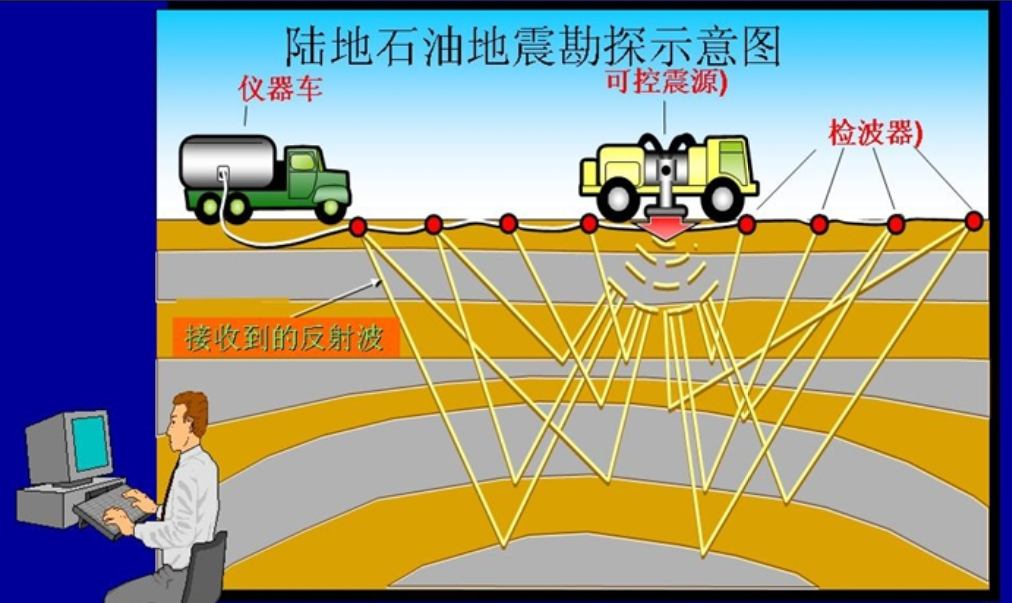
\includegraphics[width=10cm,height=5cm]{./figure/seismic.png}
  \caption{Find the support of the unknown obstacle from the knowledge of the scattered waves on a given surface.}
\end{figure}
\end{frame}
\begin{frame}
\frametitle{Direct Scattering Problem in the Half Space}
We consider elastic wave propagating in the half space with
Neumann condition(Traction Free),
\ben\label{elastic_eq}
\nabla\cdot\sigma(u_q) + \rho\omega^2u_q= -\delta_{x_s}(x)q \ \ \ \ \mbox{in }\R_+^2\bks \bar{D}\\
u_q=0 \ \ \mbox{on} \ \Ga_D  \ \ \mbox{and} \ \ \sigma(u_q)\cdot e_2=0 \ \ \mbox{on} \ \Ga_0
\een
together with the constitutive relation (Hookes law)
\ben
\sigma(u) = 2\mu\ep(u) + \lambda\div u \mathbb{I} \\
\ep(u)=\frac{1}{2}(\na u +(\na u)^T)
\een
where $\omega$ is the circular frequency, $u(x)\in\C^2$ denotes the displacement fields and $\sigma(u)$ is the stress tensor. We also need to define the surface traction $T_x^n (\cdot)$ on the normal direction n,
\ben
T_x^n u(x) := \sigma\cdot n = 2\mu\frac{\pa u}{\pa n}+\lambda n\div u + \mu n \times \curl u
\een
\end{frame}

\begin{frame}
\begin{figure}
  \centering
  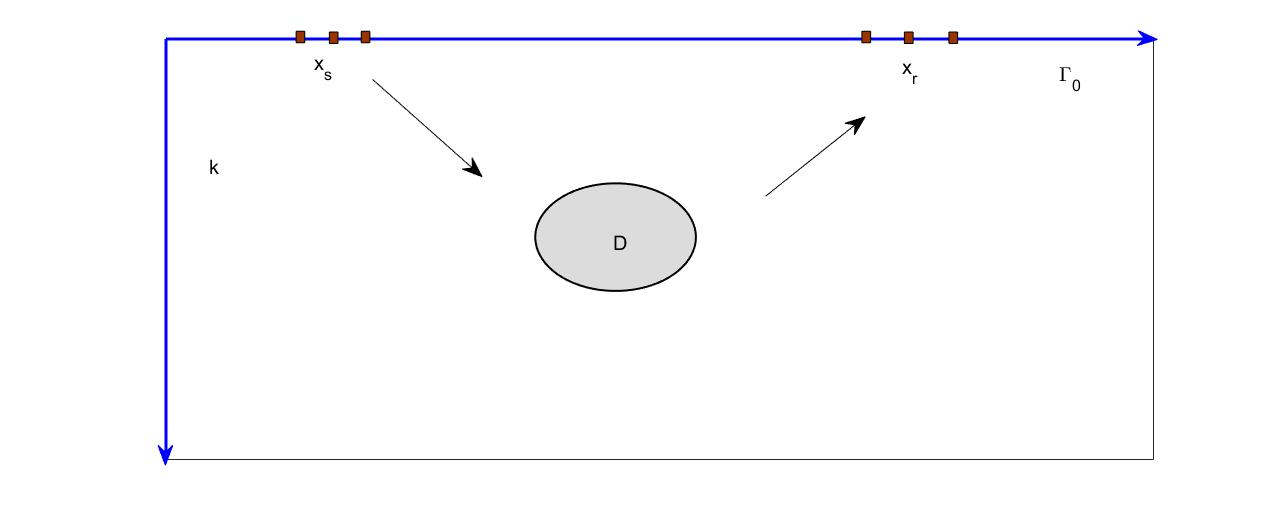
\includegraphics[width=12cm,height=8cm]{./figure/half_forward}
\end{figure}
\end{frame}


\begin{frame}
\frametitle{Green Tensor in the Half Space}
Green Tensor in the half-space with Neumann boundary  :
\ben
 \De_e \N(x;y) + \omega^2 \N(x,y) = -\mathbf{\de}_y(x) \mathbb{I} \ \ \ \ \mbox{in} \ \ \  \R^2_+ , \label{eq_n1} \\
 \sigma_x (\N(x,y))e_2 = 0 \ \ \ \ \ \ \mbox{on} \ \ \ x_2=0 \label{eq_n2}
\een
Green Tensor in the half-space with Dirichlet Boundary
\ben
 \De_e \D(x,y) + \omega^2 \D(x,y) = -\mathbf{\de}_y(x) \mathbb{I} \ \ \ \ \mbox{in} \ \ \  \R^2_+ , \label{eq_d1} \\
  \D(x,y) = 0 \ \ \ \ \ \ \mbox{on} \ \ \ x_2=0 \label{eq_d2}
\een
where $\de_y(x)$ is the Dirac source at $y \in R^2_+$ and $N(x,y)$, $\D(x,y)$ are $\mathbb{C}^{2\times2}$ matrixes.

\vspace{1cm}

\textbf{Remark}: we will assume that for $z\in\mathbb{C}$, $z^{1/2}$ is the analytic branch of $\sqrt{z}$ such that $\Im (z^{1/2})\geq0$.
\end{frame}


\begin{frame}
\frametitle{Green Tensor in Frequency Domain after Fourier Transformation}
\ben
\hat \N(\xi,x_2;y_2) = \hat \G(\xi,x_2;y_2)  -\hat \G(\xi,x_2;-y_2) + \hat \N_c(\xi,x_2;y_2)
\een
\ben
\hat
\N_c(\xi,x_2;y_2) = &=& \frac{\i}{\omega^2 \delta(\xi)} \Bigg\{ A(\xi)e^{\i\mu_s(x_2+y_2)}+B(\xi)e^{\i\mu_p(x_2+y_2)}\\ \nn
&&+C(\xi)e^{\i\mu_s x_2+\mu_p y_2}+D(\xi)e^{\i\mu_p x_2+\mu_s y_2}\Bigg\}
\een
where $\G(x,y)$ is the fundamental solution of elastic equation and
\ben
&&{A(\xi)} =
\left( \begin{array}{ll}
	\mu_s\beta^2 & -4\xi^3\mu_s\mu_p \\
	-\xi\beta^2  & 4\xi_4\mu_p
\end{array} \right)\ \ \ \ \ \
{B(\xi)} =
\left( \begin{array}{ll}
	4\xi^4\mu_s & \xi\beta^2 \\
	4\xi^3\mu_s\mu_p  & \mu_p\beta^2
\end{array} \right) \\
&&{C(\xi)} =
\left( \begin{array}{ll}
	2\xi^2\mu_s\beta & -2\xi\mu_s\mu_p\beta \\
	-2\xi^3\beta  & 2\xi^2\mu_p\beta
\end{array} \right)\ \
{D(\xi)} =
\left( \begin{array}{ll}
	2\xi^2\mu_s\beta & 2\xi^3\beta \\
	2\xi\mu_s\mu_p\beta  & 2\xi^2\mu_p\beta
\end{array} \right)
\een
and  $\mu_\alpha=(k_\alpha^2-\xi^2)^{1/2}$, $\alpha\in\{s,p\}$, $\beta(\xi)=k_s^2-2\xi^2$, $\delta(\xi)=\beta^2+4\xi^2\mu_s\mu_p $.
\end{frame}


\begin{frame}
\frametitle{Dirichlet Green Tensor in Frequency Domain after Fourier Transformation}
\ben
\hat \D(\xi,x_2;y_2) = \hat \G(\xi,x_2;y_2)  -\hat \G(\xi,x_2;-y_2) + \hat M(\xi,x_2;y_2)
\een
\ben
\hat
{M}(\xi,x_2;y_2)&=& \frac{\i}{\omega^2 \gamma(\xi)} \Bigg\{ A(\xi)e^{\i\mu_s(x_2+y_2)}+B(\xi)e^{\i\mu_p(x_2+y_2)}\\ \nn
&&-A(\xi)e^{\i\mu_s x_2+\mu_p y_2}-B(\xi)e^{\i\mu_p x_2+\mu_s y_2}\Bigg\}
\een
where
\ben
&&{A(\xi)} =
\left( \begin{array}{ll}
	\xi^2\mu_s & -\xi\mu_s\mu_p \\
	-\xi^3  & \xi^2\mu_p
\end{array} \right)\ \ \ \ \ \
{B(\xi)} =
\left( \begin{array}{ll}
	\xi^2\mu_s & \xi^3 \\
	\xi\mu_s\mu_p  & \xi^2\mu_p
\end{array} \right)
\een
and $\gamma(\xi)=\xi^2+\mu_s\mu_p$.
\end{frame}


\begin{frame}
\begin{block}{Lemme 1} \label{root_De1}
	Let \emph{Lam\'{e}} constant $\lambda, \mu \in \R^+$, then the Rayleigh equation $\delta(\xi) = 0$ has only two roots denoted by $\pm k_R$ in complex plane. Morever, $k_R > k_s > k_p, \ k_R\in\R$ and $k_R$ is called Rayleigh wave number.
\end{block}

 Using Cauchy integral theorem, we carry out:
\begin{block}{Formula 1}
\begin{tiny}
\ben
\N(x,y)= \frac{1}{2\pi}\pv\int_{\R}\hat \N(\xi,x_2;y_2) e^{\i(x_1-y_1)\xi} d\xi
-\frac{\i}{2}\frac{\N_\delta(-k_R)}{\delta'(-k_R)}e^{-\i(x_1-y_1)k_R}+\frac{\i}{2}\frac{\N_\delta(k_R)}{\delta'(k_R)}e^{\i(x_1-y_1)k_R}
\een
\end{tiny}
where $\N_\delta(\xi)=\hat \N(\xi,x_2;y_2)\delta(\xi)$.
\end{block}
\end{frame}




\begin{frame}
\begin{small}
\begin{block}{Lemma 2} \label{root_Ga}
	Let \emph{Lam\'{e}} constant $\lambda, \mu \in \C$ and $\Im(k_s)\geq0, \Im(k_p)\geq0$, then equation $\gamma(\xi) = 0$ has no root in complex plane.
\end{block}
\begin{block}{Formula 2}
Let $\T_D(x,y)$ denote the traction of $\D(x,y)$ in direction $e_2$ with respect to $x$ such that $\T_D(x,y)e_i=\
\sigma_x(\D(x,y)e_i)e_2$.
\ben
\T_D(x,y)&=&\T(x,y)-\T(x,y')+\frac{1}{2\pi}\int_{\R}\hat \T_M(\xi,x_2;y_2) e^{\i(x_1-y_1)\xi}d\xi
\een
and
\ben
\hat
\T_M(\xi,x_2;y_2)&=& \frac{\mathrm{\mu}}{\omega^2 \gamma(\xi)} \Bigg\{ E(\xi)e^{\i\mu_s(x_2+y_2)}+F(\xi)e^{\i\mu_p(x_2+y_2)}\\ \nn
&&-E(\xi)e^{\i\mu_s x_2+\mu_p y_2}-F(\xi)e^{\i\mu_p x_2+\mu_s y_2}\Bigg\}
\een
where
\ben
&&{E(\xi)} =
\left( \begin{array}{cc}
	-\xi^2\beta & \xi\mu_p\beta \\
	2\xi^3\mu_s & -2\xi^2\mu_s\mu_p
\end{array} \right)\ \ \ \
{F(\xi)} =
\left( \begin{array}{cc}
	-2\xi^2\mu_s\mu_p & -2\xi^3\mu_p \\
	-\xi\mu_s\beta  & -\xi^2\beta
\end{array} \right)
\een
\end{block}
\end{small}
\end{frame}


\begin{frame}
\frametitle{Inverse Scarttering Problem}
\begin{columns}
\begin{column}{.5\textwidth}

\begin{tiny}
\begin{eqnarray*}
\left\{
\begin{array}{lll}
\nabla\cdot\sigma(u_q) + \rho\omega^2u_q= -\delta_{x_s}(x)q \ \ \ \ &in&\R_+^2\bks \bar{D}\\
u_q=0 \ \  \ \ \ \ \ \ \ &on& \ \Ga_D  \ \ \\
\sigma(u_q)\cdot e_2=0 \ \ &on& \ \Ga_0
\end{array}
\right.
\end{eqnarray*}
\end{tiny}
\small{satisfies the generalized radiation condition}
\end{column}

\begin{column}{.5\textwidth}
\begin{figure}
  \centering
  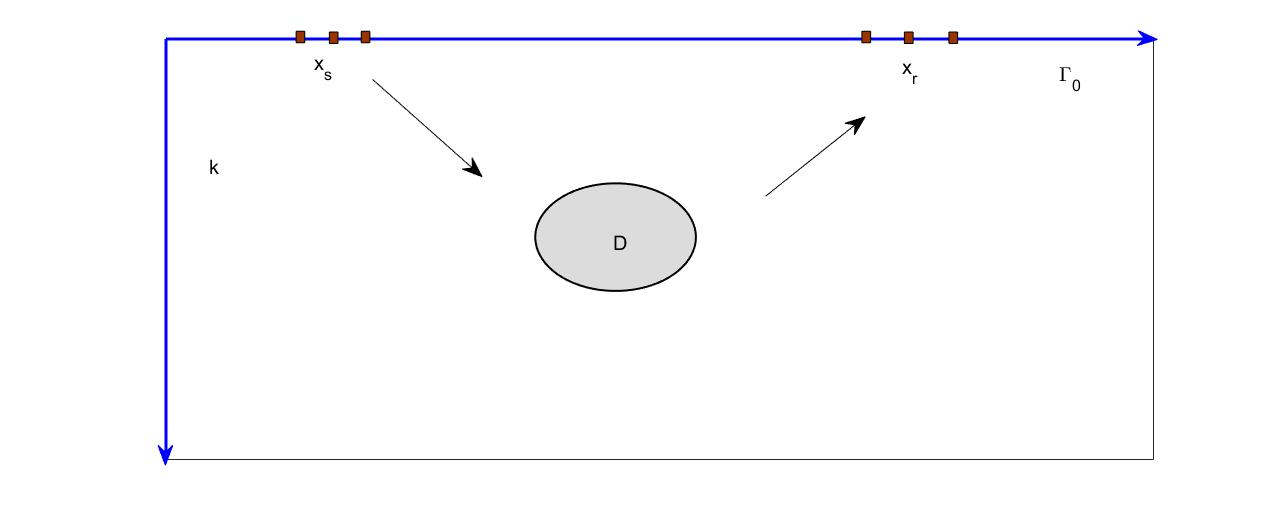
\includegraphics[width=6cm,height=3cm]{./figure/half_forward}
\end{figure}
\end{column}
\end{columns}
\begin{block}{Direct Problem}
To determine the scattering wave field $u^s(x,x_s)=u(x,x_s)-u^i(x,x_s)$ from the given incident field $u^i(x,x_s)=\N(x,x_s)$,
the differential equation governing the wave motion and the information of obstacle.
\end{block}
\begin{block}{Inverse problem}
To determine the location, size, sharp of the obstacle by the measured field $u^s(x,x_s)$ on $x_r$
\end{block}
\end{frame}


\begin{frame}
\frametitle{Algorithms of inverse obstacle problem}
\begin{columns}

\column{.5\textwidth}

\begin{block}{Direct Imaging Method}
\begin{itemize}
  \item Linear Sample MethodFactorization methodPoint source method
  \item MUltiple SIgnal Classification
  \item Prestack depth migration\textcolor{blue}{Reverse Time Migration}
\end{itemize}

\end{block}
\begin{block}{Feature}
  Fast computationDifficult mathematics analysis
\end{block}
\column{.5\textwidth}

\begin{block}{Iterative Method}
\begin{itemize}
  \item Differential semblance optimization
  \item Full waveform inversion
  \item Recursive linearization  algorithm
\end{itemize}
\end{block}
\begin{block}{Feature}
 Need prior information, Difficult to convergence, Provide quantitative information
\end{block}
\end{columns}
\begin{block}{Reverse Time Migration}
 \begin{itemize}
 \item Do not require any priori information
of the physical properties of the obstacle such as penetrable or non-penetrable, and
for non-penetrable obstacles, the type of boundary conditions on the boundary of the
obstacle.
  \item The previous analysis of the migration
method is usually based on the high frequency assumption so that the geometric optics
approximation can be used.
\end{itemize}
\end{block}
\end{frame}

\section{Reverse Time Migration}


\begin{frame}
\frametitle{Reverse Time MigrationMathematics Framework}
\begin{small}
\begin{block}{Acoustic, electromagnetic, elastic wave in the Full space}
\begin{enumerate}
  \item Chen J, Chen Z, Huang G. {\it Reverse time migration for extended obstacles: acoustic waves [J]}. Inverse Problems. 2013, 29(8):645-648
  \item Chen J, Chen Z, Huang G. {\it Reverse time migration for extended obstacles: Electromagnetic waves[J]}. Scientia Sinica, 2015, 29(8):085005.
  \item Chen Z, Huang G. {\it Reverse time migration for extended obstacles: Elastic waves (in Chinese)[J]}. Science China Mathematics, 2015, 45(8):1103-1114.
\end{enumerate}
\end{block}
\begin{block}{Planar acoustic waveguide}
\begin{enumerate}
  \item Chen Z M, Huang G H. {\it Reverse time migration for reconstructing extended obstacles in planar acoustic waveguides[J]}. Science China Mathematics, 2015, 58(9):1811-1834.
\end{enumerate}
\end{block}

\begin{block}{Acoustic in the Half space}
\begin{enumerate}
  \item Chen Z, Huang G. {\it Reverse time migration for reconstructing extended obstacles in the half space[J].} Inverse Problems, 2015, 31(5):055007 (19pp).
\end{enumerate}
\end{block}

\begin{block}{Phaseless Algorithm}
\begin{enumerate}
  \item Chen Z, Huang G. {\it Phaseless Imaging by Reverse Time Migration: Acoustic Waves[J]. } Numerical Mathematics Theory Methods and Applications, 2017, 10(1):1-21.
%  \item Chen Z, Huang G. {\it A Direct Imaging Method for Electromagnetic Scattering Data without Phase Information[J]. }Siam Journal on Imaging Sciences, 2016, 9(3).
%  \item Chen Z, Fang S, Huang G. {\it A Direct Imaging Method for the Half-Space Inverse Scattering Problem with Phaseless Data[J].} Inverse Problems and Imaging, 2017, 11(5).
\end{enumerate}
\end{block}
\end{small}

\end{frame}

\begin{frame}
\begin{figure}
  \centering
  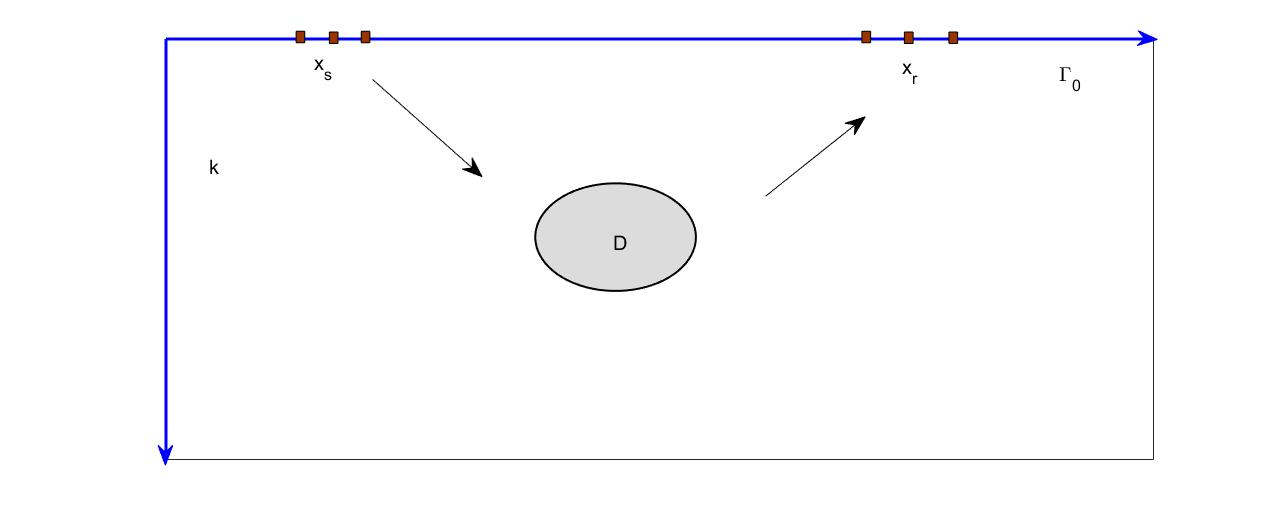
\includegraphics[width=12cm,height=8cm]{./figure/half_forward}
\end{figure}
\end{frame}
\begin{frame}
\frametitle{RTM Algorithm}
Given the data $u_k^s(x_r,x_s)$, $k=1,2$ which is the measurement of the scattered field at $x_r$ when the source is emitted at $x_s$ along the  polarized direction $e_k$, $s=1,\dots, N_s$ and $r=1,\dots,N_r$.
\be\label{cor1}
I_d(z)=\Im\sum_{k=1}^{2}\left\{\frac{|\Gamma_0^d|}{N_s}\sum^{N_s}_{s=1}\sum_{i=1}^{2}[\sigma_{x_s}(\D(x_s,z)e_i)e_2\cdot e_k][v_k(z,x_s)\cdot e_i]\right\}. \ \ z\in \Omega
\ee
where $v_k(z,x_s)$ satisfy the following scattering elastic equation:
\ben
\Delta_e v_k(z,x_s) + \omega^2 v_k(z,x_s) =0 \qquad\mbox{\rm in } \R^2_+ \\
v_k(z,x_s)=\frac{|\Ga_0^d|}{N_r}\sum_{r=1}^{N_r}\overline{u^s_k(x_r,x_s)}\delta_{x_r}(z) \ \ \ \ \mbox{\rm on}  \ \ \Ga_0
\een
By letting $N_s,N_r\to\infty$, we know that (\ref{cor1}) can be viewed as an approximation of the following continuous integral:
\ben
\hat{I}_d(z)=\Im\sum_{q=e_1,e_2}\int_{\Gamma_0^d}\int_{\Gamma_0^d}\,
[\T_D(x_s,z)^Tq][\T_D(x_r,z)^T\overline{u^s_q(x_r,x_s)}]\,ds(x_r)ds(x_s).
\een
where $z\in\Om$.
\end{frame}


\section{Resolution Analysis}
\begin{frame}
\frametitle{Point Spread Function}
The point spread function measures the resolution to find a point source. Given the $\N(x,y)$ on $\Gamma_0^d=\{(x_1,x_2)^T\in\Gamma_0, \  x_1\in(-d,d)\}$ with the source $y\in \R_+^2$, we define the PSF as the back-propagated field $\J_d(x,y)$.
\ben
\De_e \J_d(x,y) + \omega^2 \J_d(x,y) = -\mathbf{\de}_y(x) \mathbb{I}  \ \ \ in \ \  \R^2_+ , \label{eq_d3} \ \ \
  \J_d(x,y) = \N(x,y)\chi_{(-d,d)} \ \ \ \ \ \ on \ \ \ \Gamma_0
\een
By integral representation
\ben
\J^{ij}_d(z,y):&=&e_i\cdot \J_d(z,y) e_j \\
&=&\int_{\Gamma_0^d} \ \sigma_x(\D(x,z)e_i)e_2\cdot\overline{\N(x,y)}e_j ds(x) \\ \label{fullpsf}
&=&\int_{-d}^d \ \sigma_x(\D(x_1,0;z_1,z_2)e_i)e_2\cdot\overline{\N(x_1,0;y_1,y_2)}e_j dx_1
\een
\end{frame}

\begin{frame}
\frametitle{Numerical test: PSF}
\begin{figure}[h]
  \centering
  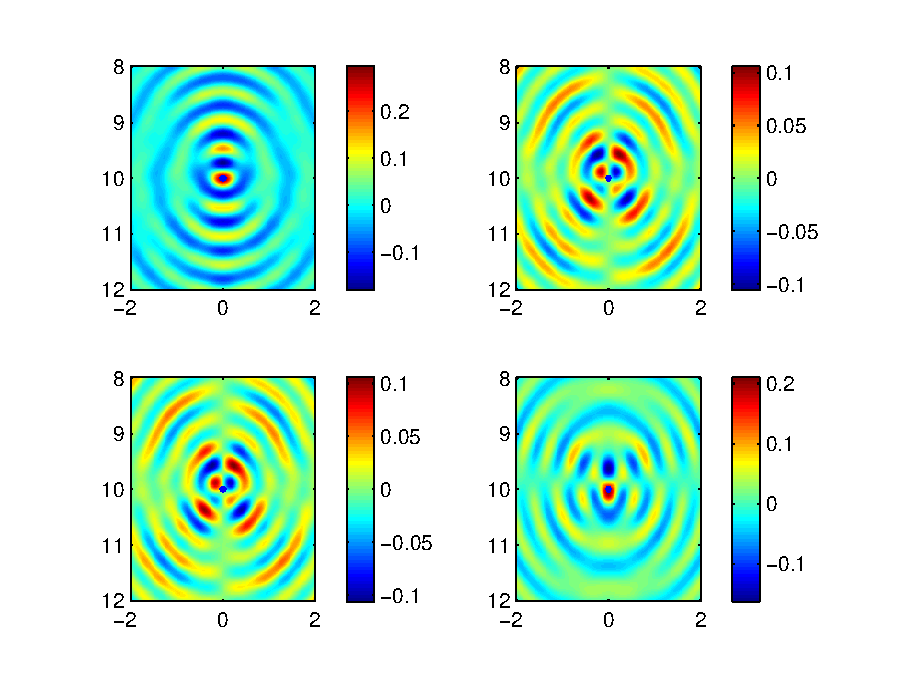
\includegraphics[width=0.8\textwidth]{./psf/J.eps}
  \caption{The figures on the diagonal line show that psf have peaks on the point x=y}\label{fig_wgout_ex1}
\end{figure}
\end{frame}

\begin{frame}
\frametitle{Analysis of PSF}
\begin{block}{Hypothesis}
 We assume the obstacle $D\subset\Omega$ and there exist constants $0<c_1<1,c_2>0,c_3>0$ such that
\ben\label{convention_2}
h<d, \ \ |x_1|\leq c_1 d , \ \ |x_1-y_1|\leq c_2 h , \ \
|x_2|\leq c_3 h    \ \ \ \forall x,y \in \Omega
\een
\end{block}
\begin{block}{Theorem 1}
	Let $k_s h>1$. For any $z,y\in\Om$, PSF can be reprsented by  $J_d(z,y)=\F(z,y)+\R(z,y)$ and it satisfy that
	\ben
	|\R_{ij}(z,y)|+k_s^{-1}|\na_y \R_{ij}(z,y)|\leq \frac{C}{\mu}(\frac{1}{(k_s h)^{\frac{1}{2n^*}}}
    +k_she^{-k_s h\sqrt{\kappa_R^2-1}}) \\ +\frac{C}{\mu} ((\frac{h}{d})^{2}+\frac{(k_s h)^{1/2}}{ e^{k_s h\sqrt{\kappa_R^2-1}}}(\frac{h}{d})^{1/2})
	\een
	uniformly for $z,y\in\Om$. Here $\kappa_R:=k_R/k_s$ and the constant C may dependent on $k_s d_D$ and $\kappa:=k_p/k_s$, but is independent of $k_s$, $k_p$, h, $d_D$.
\end{block}
\end{frame}

\begin{frame}
\frametitle{Main Term of PSF}
Based on the above argument, we know that $\R(z,y)$ becomes small when z,y move away from $\Gamma_0$ and $d\gg h$. Our goal is to show $\F(z,y)$ has the similar decay to the elastic fundamental solution $\Im\Phi(z,y)$ as $|z-y|\to\infty$.
\begin{block}{Theorem 2}
	For any $z,y\in \R_+^2$, when $z=y$
	\ben
	|\Im \F_{ii}(z,y)| \geq \frac{1}{4(\lambda+2\mu)} \ , \ i =1 ,2 \\
	\Im \F_{12}(z,y) = \Im \F_{21}(z,y) =0
	\een
	and for $z\neq y$
	\ben
	|\F_{ij}(z,y)|&\le \frac{C}{\mu}[(k_s|z-y|)^{-1/2})+(k_s|z-y|^{-1})]
	\een
	where constant $C$ is only dependent on $\kappa:=k_p/k_s$.
\end{block}
\end{frame}
\begin{frame}
Now, We turn to  study the resolution of the function $\hat{I}_d(z)$. To do this, we first show the difference between the half space scattering solution and the full space scattered solution is small if the scatterer is far away from the boundary $\Ga_0$.
\begin{block}{Theorem 3}
	Let $g\in H^{1/2}(\Ga_D)$ and $\u_1,\u_2$ be the scattering solution of following problems:
	\ben\label{elas_r1}
	\Delta_e \u_1 + \omega^2 \u_1=0 \qquad\mbox{\rm in } \R^2_+\bks \bar{D}\\
	\u_1= g \ \ \ \ \mbox{\rm on } \Ga_D  \label{elas_rbd}\\
	\sigma(\u_1)e_2=0 \ \ \ \ \mbox{\rm on} \ \ \Ga_0 \label{elas_rb0}
	\een
	and
	\ben {\label{elas_r2}}
	\Delta_e \u_2 + \omega^2 \u_2=0 \qquad\mbox{\rm in } \R^2\bks \bar{D}\\
	\u_2 = g \ \ \ \ \mbox{\rm on } \Ga_D  \label{elas_rbd2}
	\een
	Then there exits a constant C independent of $k_s$, $k_p$, such that

    \begin{small}
	\ben
	\|\sigma_x(\u_1-\u_2)\nu\|_{H^{-1/2}(\Gamma_D)}
	\leq \frac{C}{\mu}(1+\|T_f\|)(1+\|T_h\|)(1+k_s d_D)^2\epsilon_1(k_s h)\|g\|_{ H^{1/2}(\Ga_D)}
	\een
    \end{small}
\end{block}

\end{frame}

\begin{frame}
\frametitle{Resolution Analysis}
\begin{block}{Theorem 4}
	For any $z\in\Omega$, let $\Psi(y,z)\in\C^{2\times2}$ be the radiation solution of the problem:
	\ben
	& & \Delta_e \Psi(y,z)e_i + \omega^2\Psi e_i= 0 \ \ \ \ \mbox{in }\R_+^2\bks \bar{D} \ \ \ i=1,2 \\
	& &\Psi(y,z)= -\overline{\F(z,y)} \ \ \ \ \ \ \ \mbox{on} \ \Ga_D  \\
	\een
	Then, we have
	\be\hspace{-1cm}
	\hat{I}_d(z)=\Im\int_{\Gamma_D}\sum_{i=1}^2[\sigma_y (\overline{(\F(z,y)}+\Psi(y,z))e_i)\cdot \overline{\F(z,y)}e_i]ds(y)+\W_{\hat{I}}(z)
	\ee
	where $|\W_{\hat{I}}(z)|\leq \frac{C}{\mu}(1+\|T_f\|)(1+\|T_h\|)(1+k_s d_D)^4(\epsilon_1(k_s h)+\epsilon_2(k_s h,h/d))$ uniformly for z in $\Om$.
\end{block}
\end{frame}

\section{Numerical Test}
\begin{frame}
\frametitle{Numerical Test: Different Boundary Condition}
 \begin{figure}
 	\centering
 	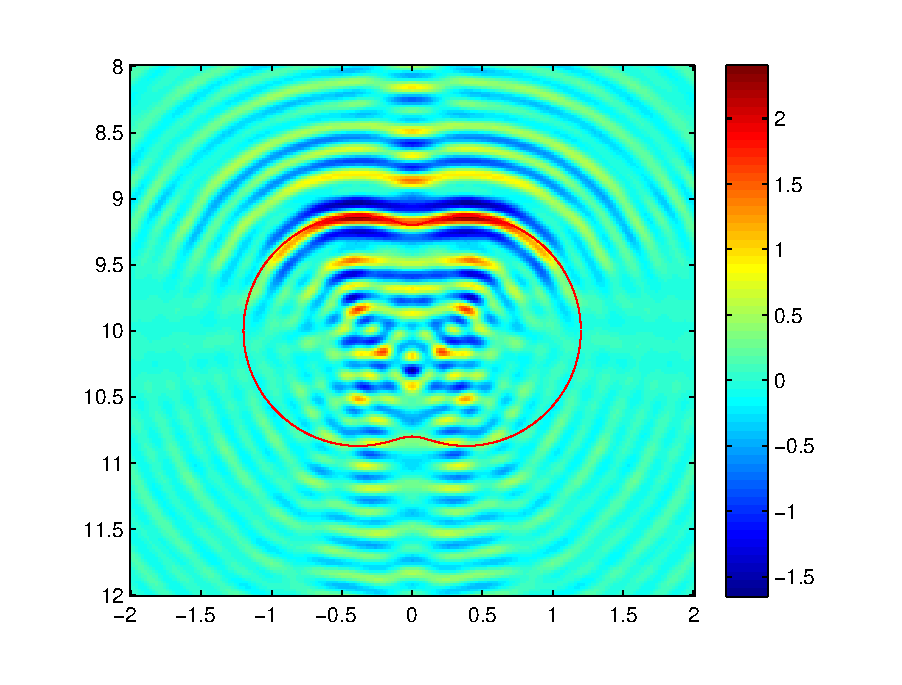
\includegraphics[width=0.24\textwidth]{./graphic/peanut_3pi.eps}
 	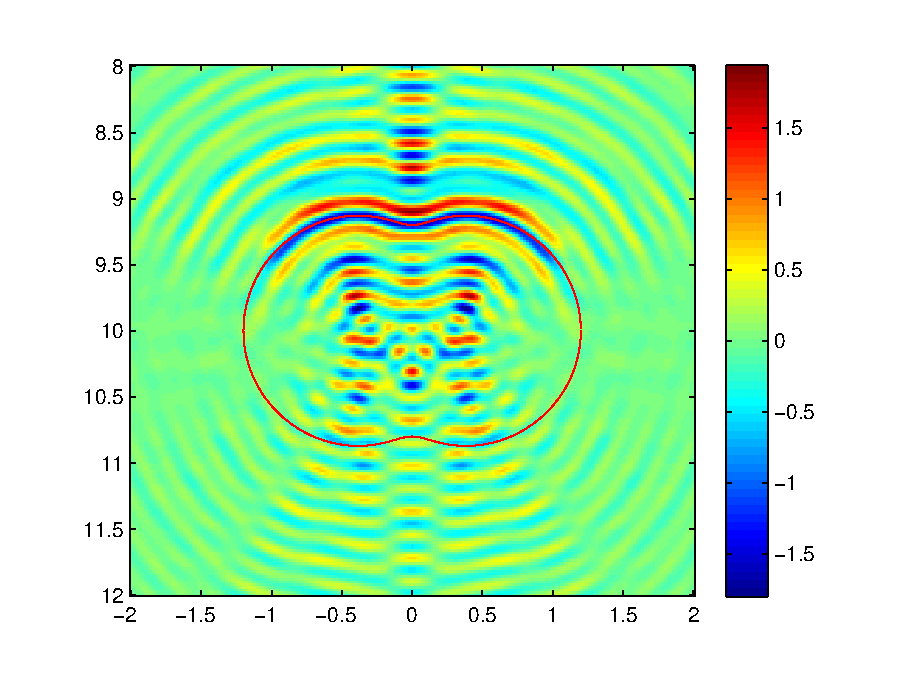
\includegraphics[width=0.24\textwidth]{./graphic/peanut_3pi_neumann.eps}
 	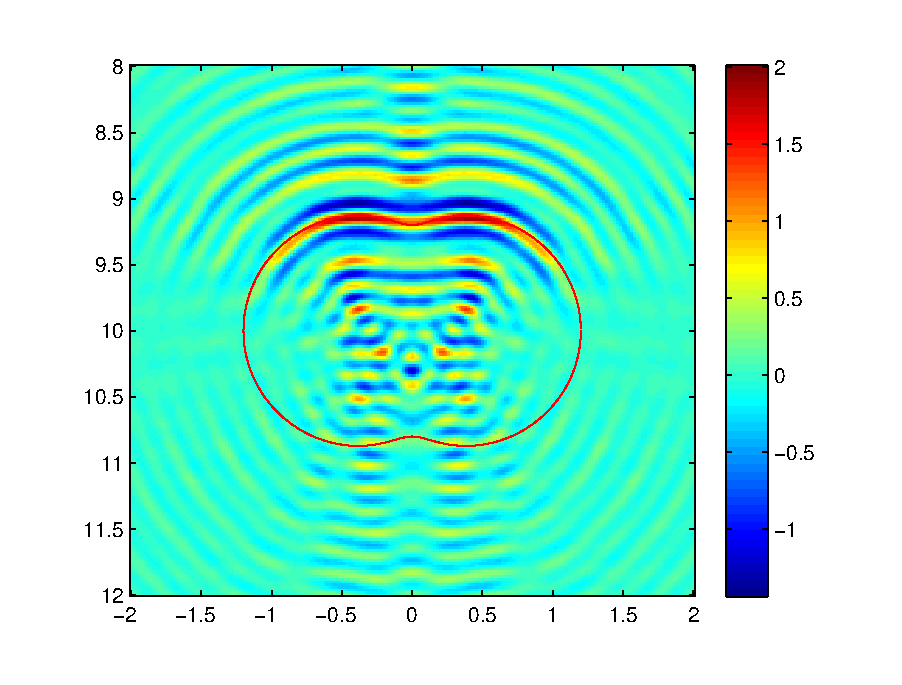
\includegraphics[width=0.24\textwidth]{./graphic/peanut_3pi_impedance_1.eps}
 	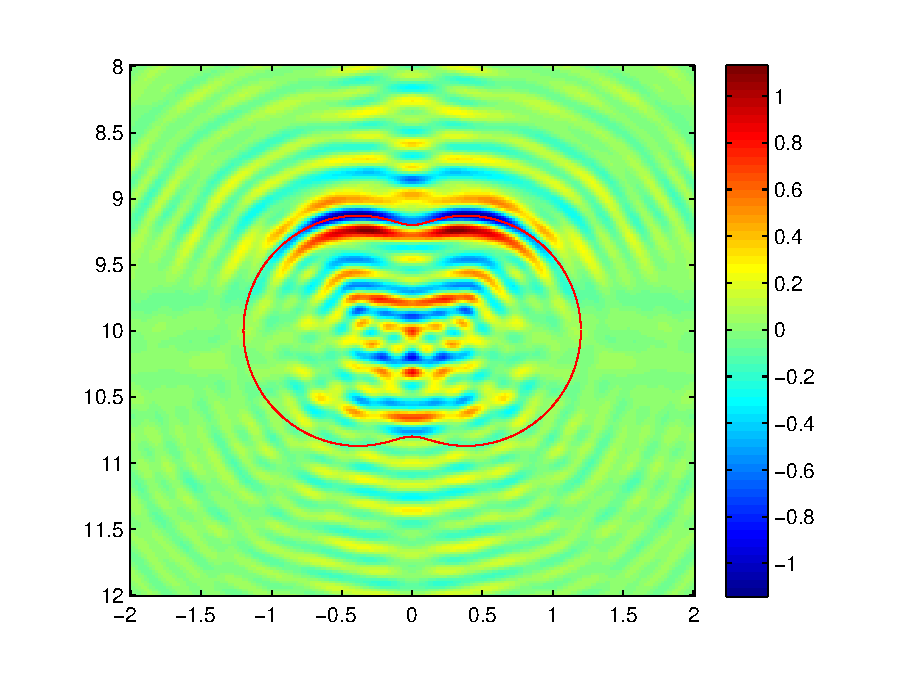
\includegraphics[width=0.24\textwidth]{./graphic/peanut_3pi_transmission.eps}\\
    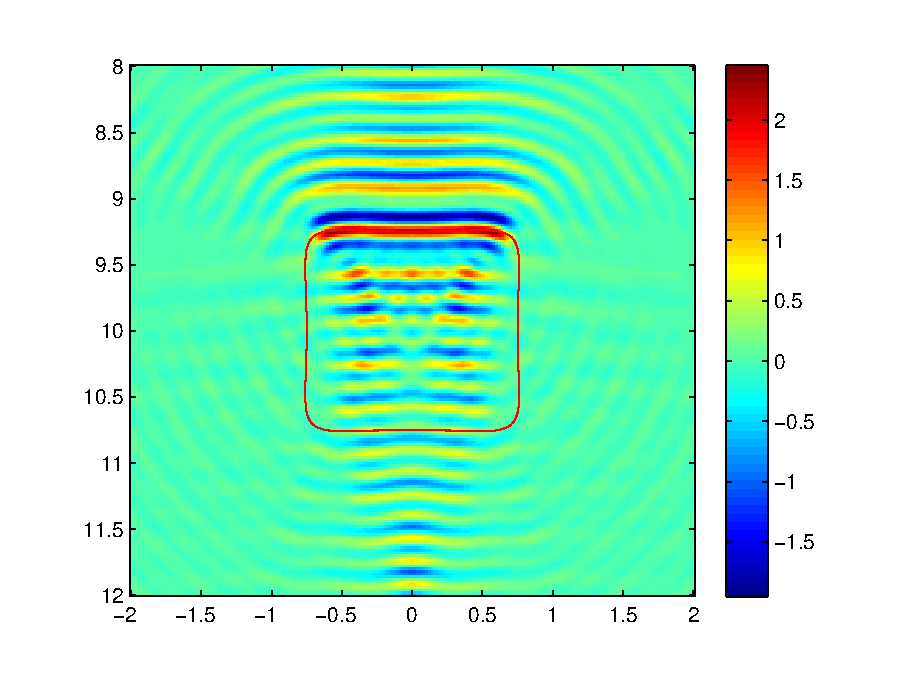
\includegraphics[width=0.24\textwidth]{./graphic/rectangle_3pi.eps}
 	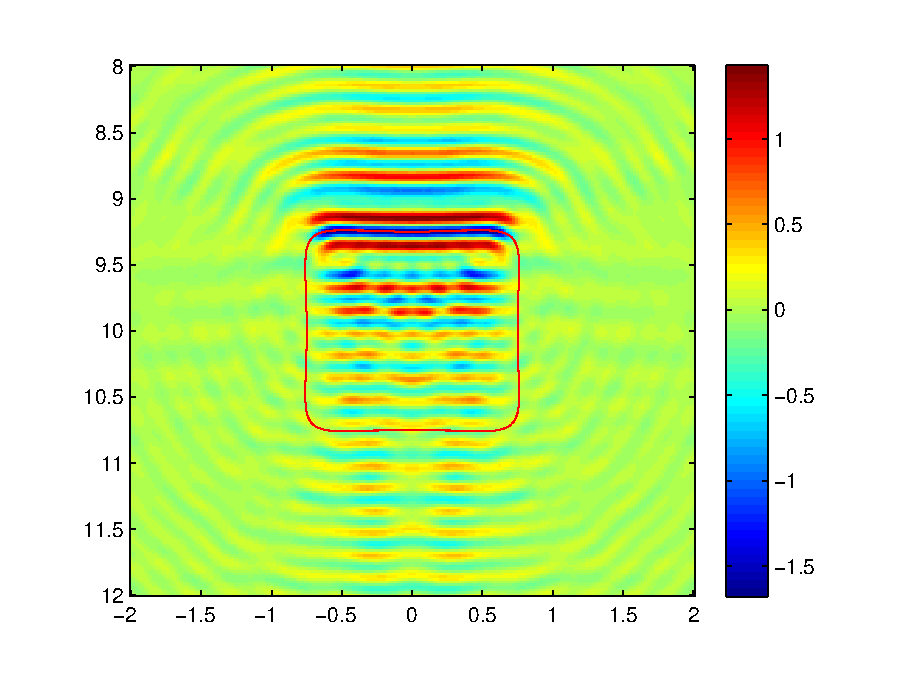
\includegraphics[width=0.24\textwidth]{./graphic/rectangle_3pi_neumann.eps}
 	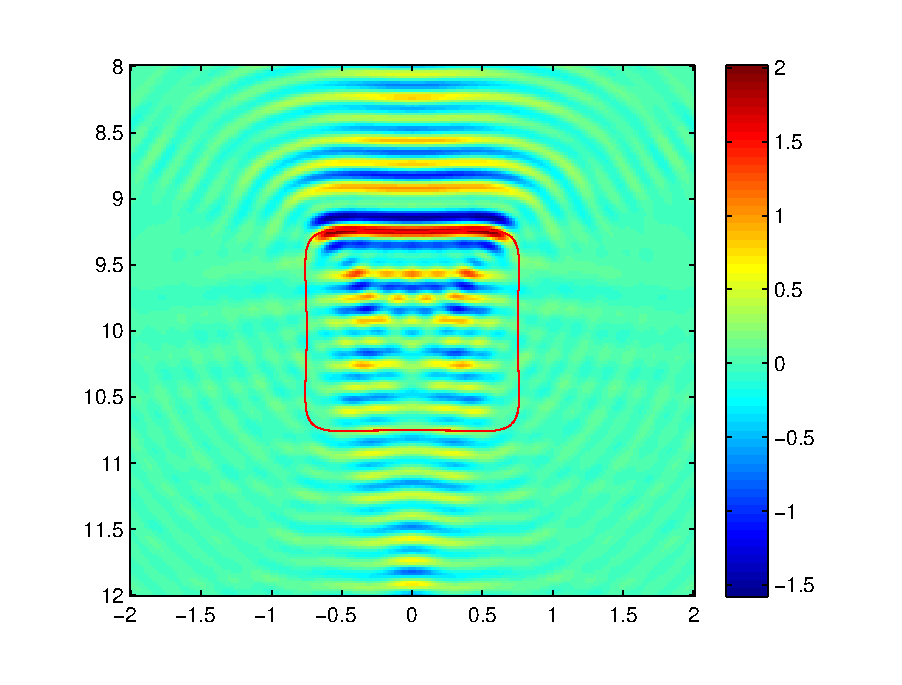
\includegraphics[width=0.24\textwidth]{./graphic/rectangle_3pi_impedance_1.eps}
 	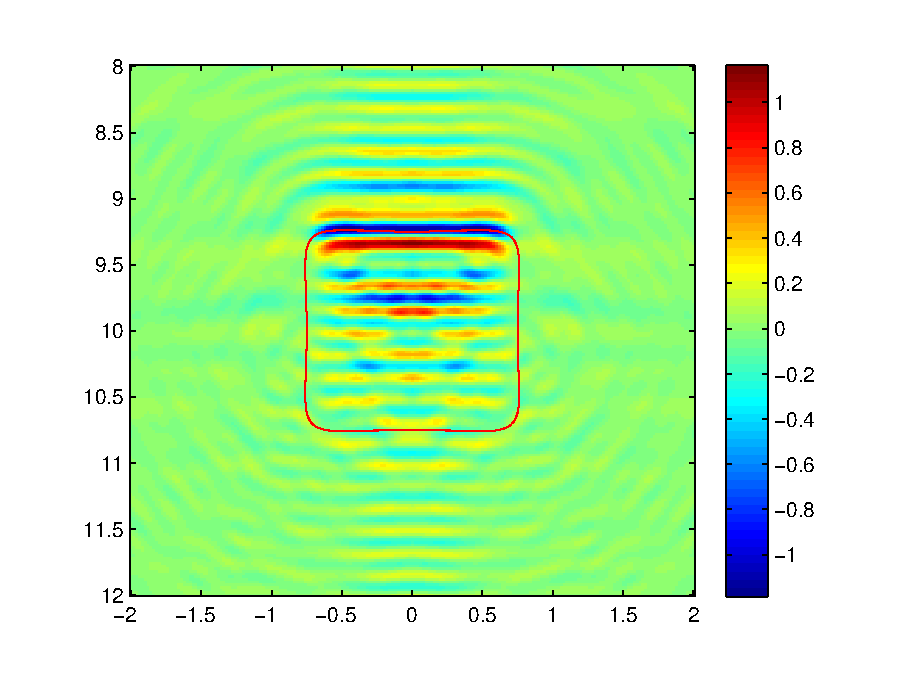
\includegraphics[width=0.24\textwidth]{./graphic/rectangle_3pi_transmission.eps}
 	\caption{Example 1: From left to right: imaging results of a Dirichlet, a Neumann, a Robin bounday with impedance $\eta(x)=1$, and a penetrable obstacle with diffractive index $n(x)=0.25$}
 \end{figure}
\end{frame}
\begin{frame}
\frametitle{Numerical Test: Different Sharp}
\begin{figure}[h]
	\centering
	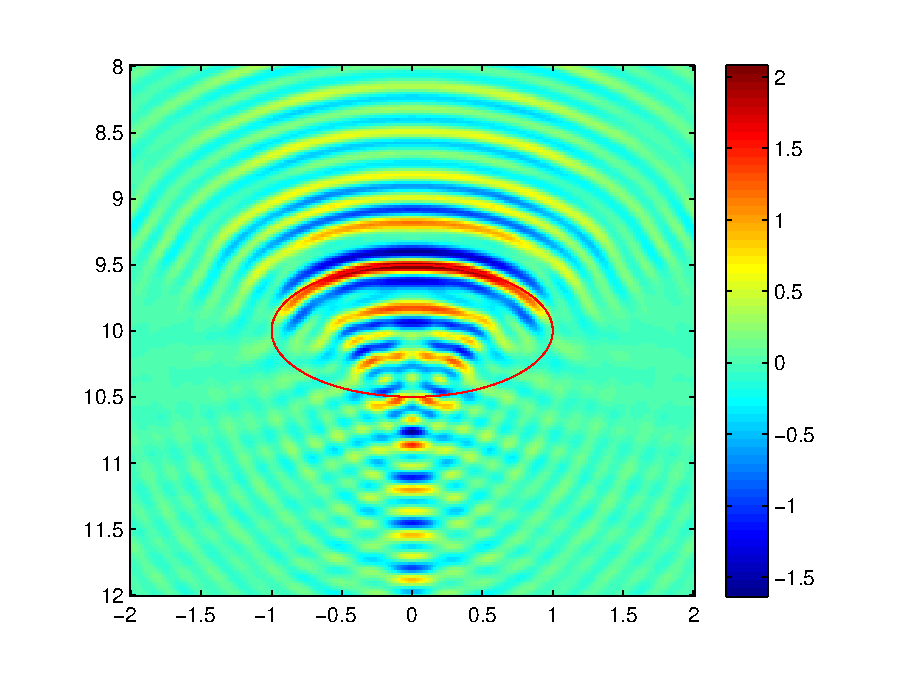
\includegraphics[width=0.32\textwidth]{./graphic/circle_3pi.eps}
	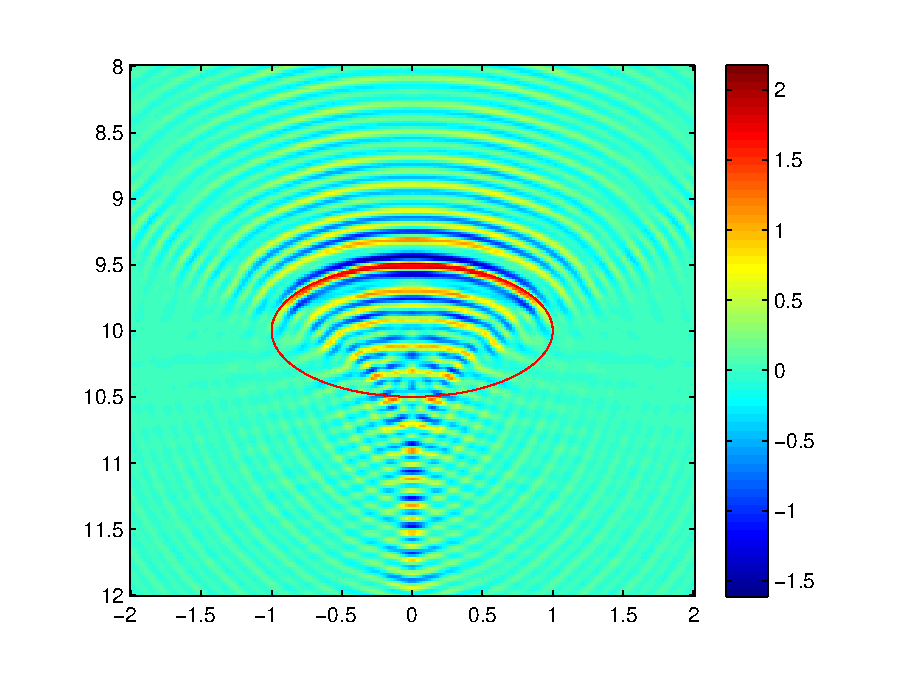
\includegraphics[width=0.32\textwidth]{./graphic/circle_5pi.eps}
	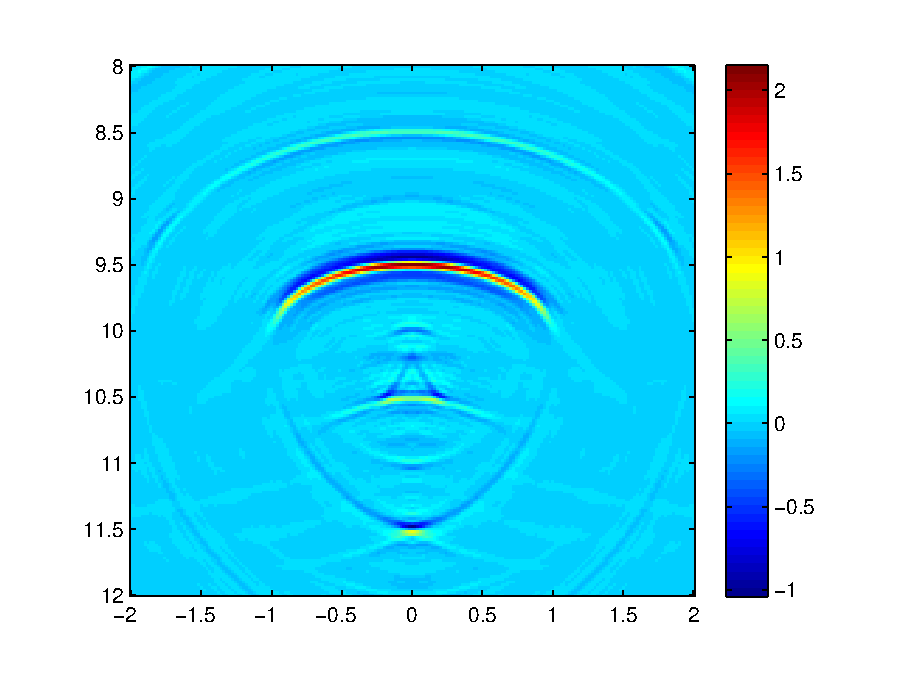
\includegraphics[width=0.32\textwidth]{./graphic/circle.eps}\\
	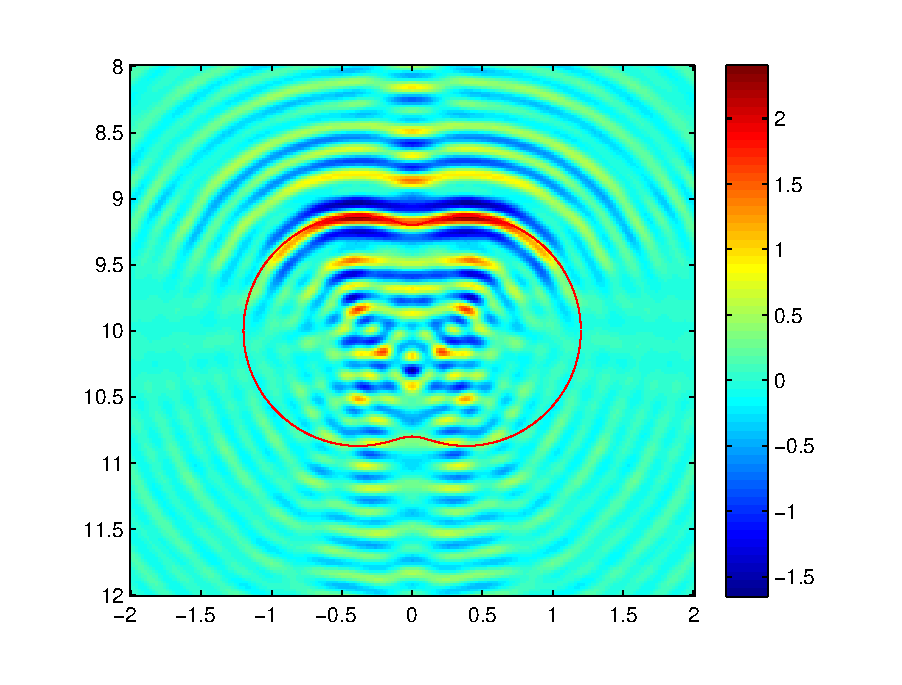
\includegraphics[width=0.32\textwidth]{./graphic/peanut_3pi.eps}
	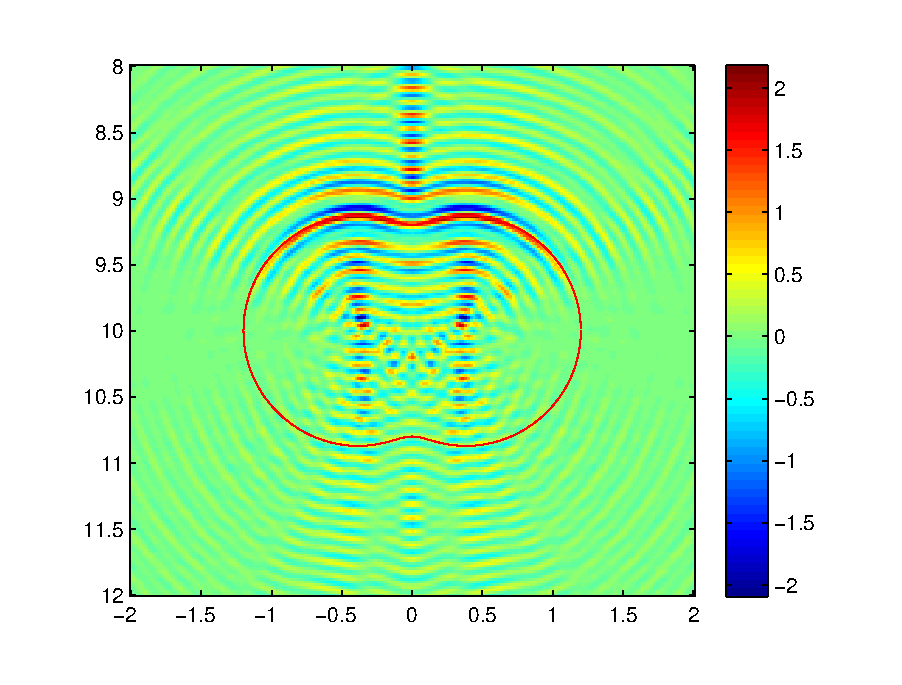
\includegraphics[width=0.32\textwidth]{./graphic/peanut_5pi.eps}
	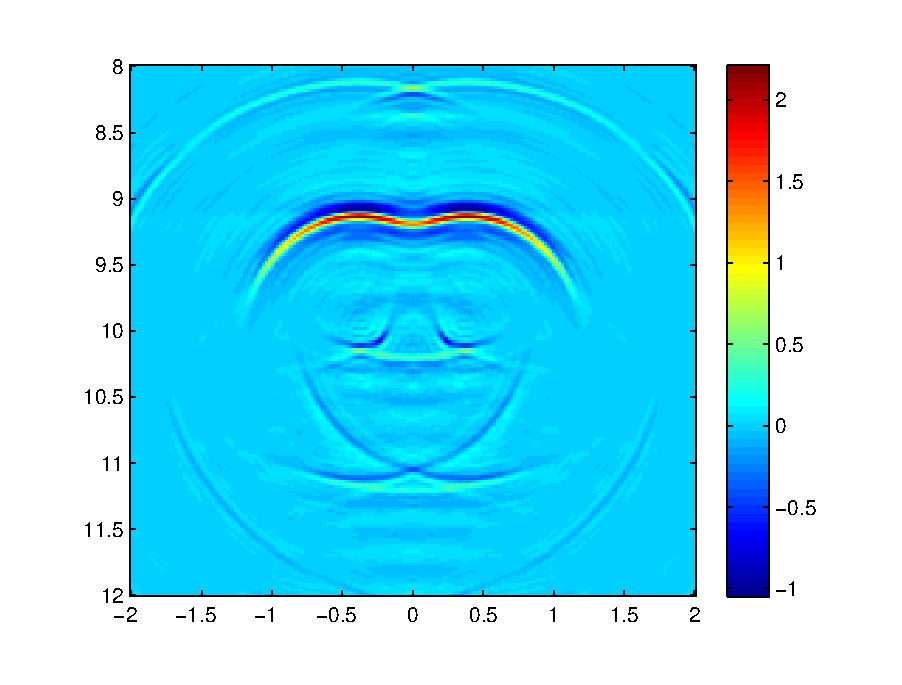
\includegraphics[width=0.32\textwidth]{./graphic/peanut.eps}
\caption{Example 2: Imaging results of clamped obstacles
		with different shapes from top to below. The left row is imaged with single frequency data where $\om=3\pi$, The middle row is imaged with single frequency data where $\om=5\pi$ and The left row is imaged with multi frequency data}
  \label{fig_wgout_ex2}
\end{figure}
\end{frame}

\begin{frame}
\frametitle{Numerical Test: Different Sharp}
\begin{figure}[h]
    \centering
	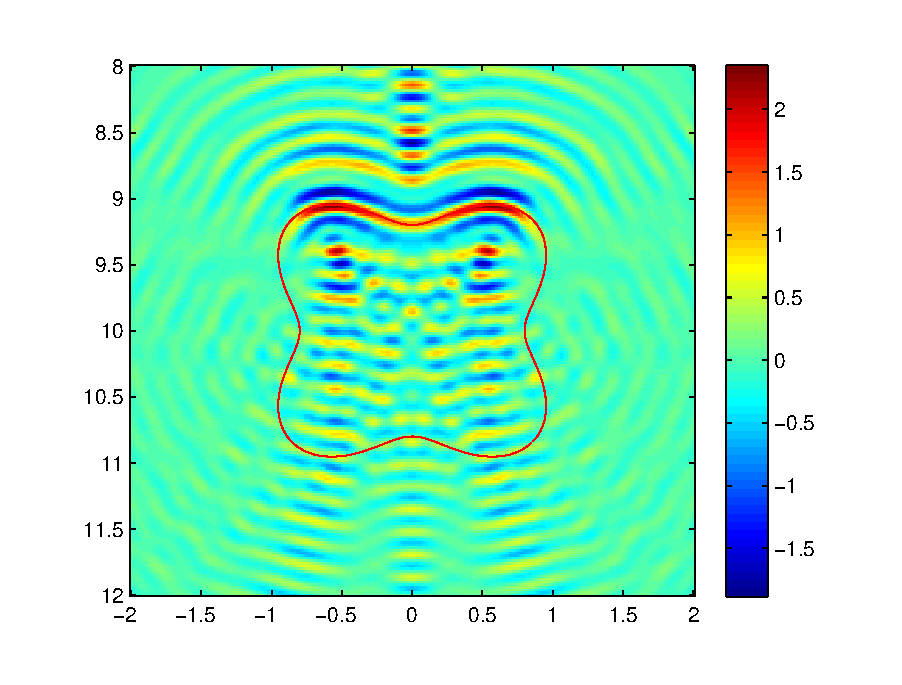
\includegraphics[width=0.32\textwidth]{./graphic/p_leaf_3pi.eps}
	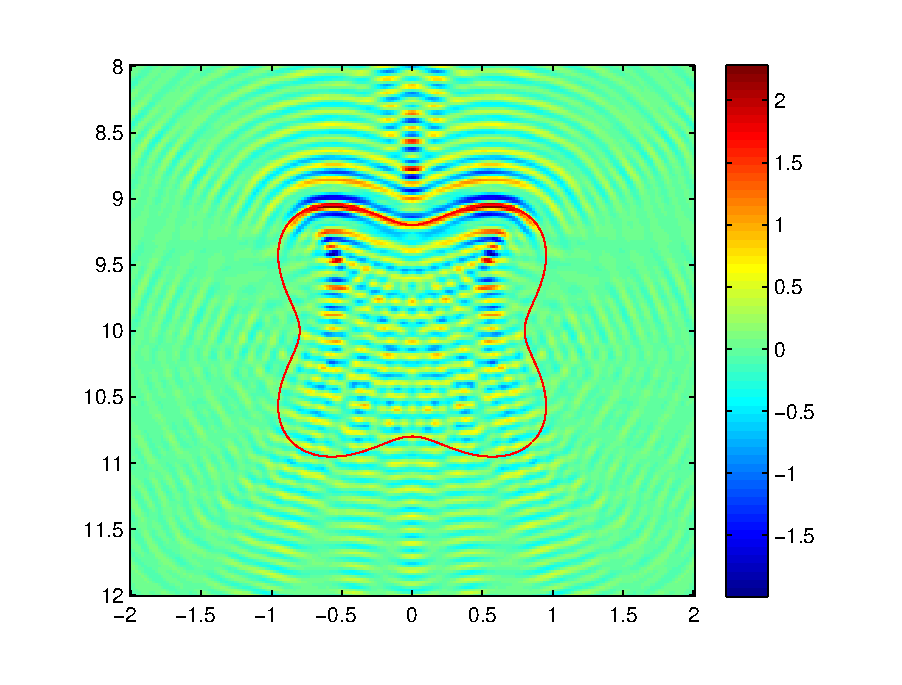
\includegraphics[width=0.32\textwidth]{./graphic/p_leaf_5pi.eps}
	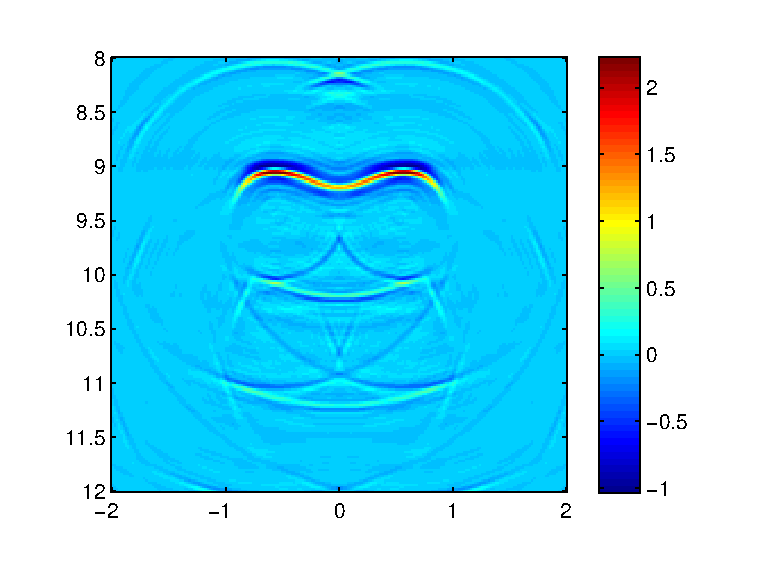
\includegraphics[width=0.32\textwidth]{./graphic/p_leaf.eps}\\
	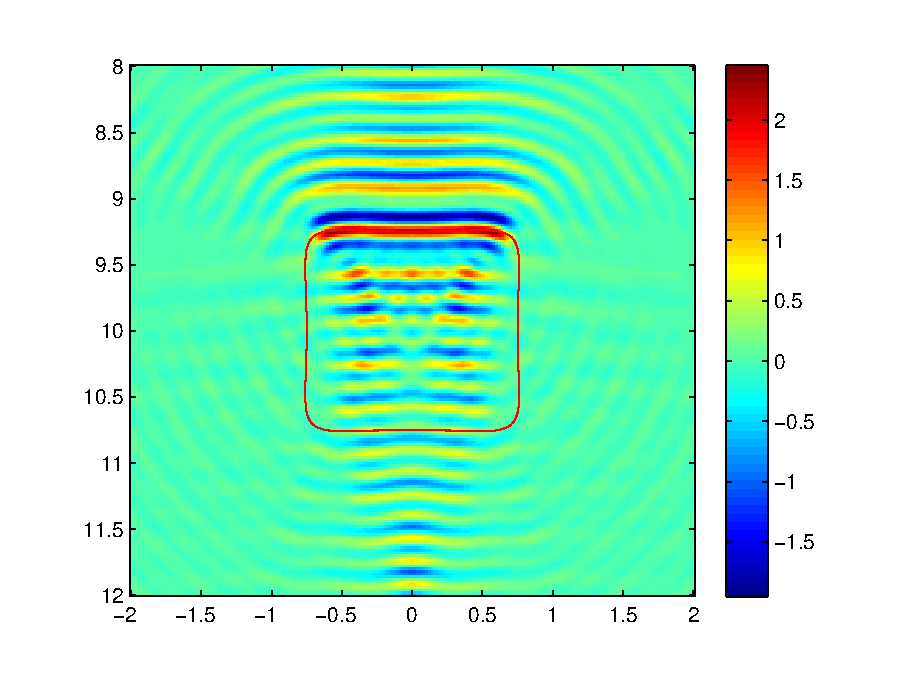
\includegraphics[width=0.32\textwidth]{./graphic/rectangle_3pi.eps}
	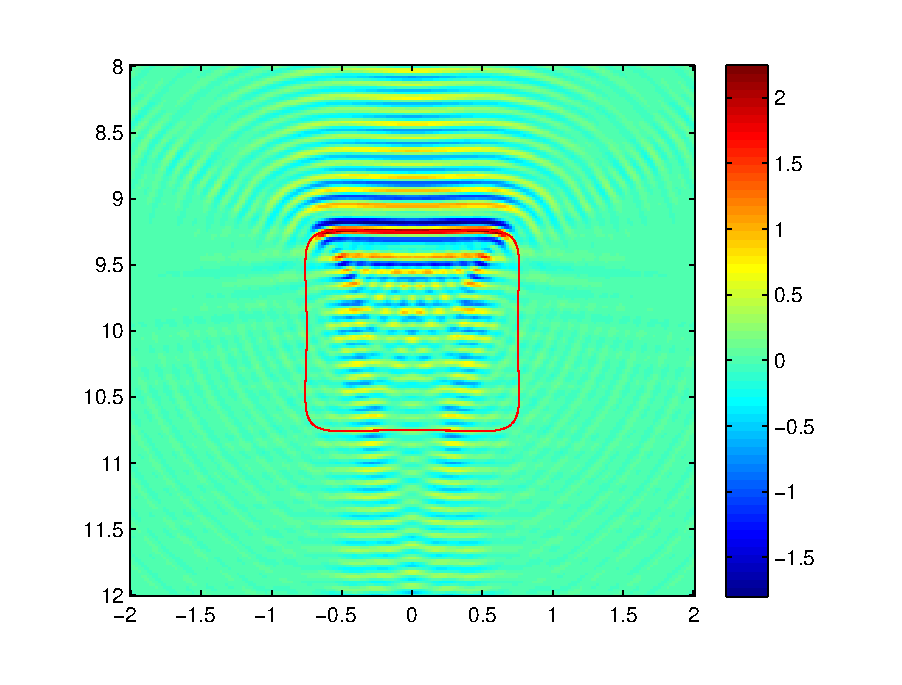
\includegraphics[width=0.32\textwidth]{./graphic/rectangle_5pi.eps}
	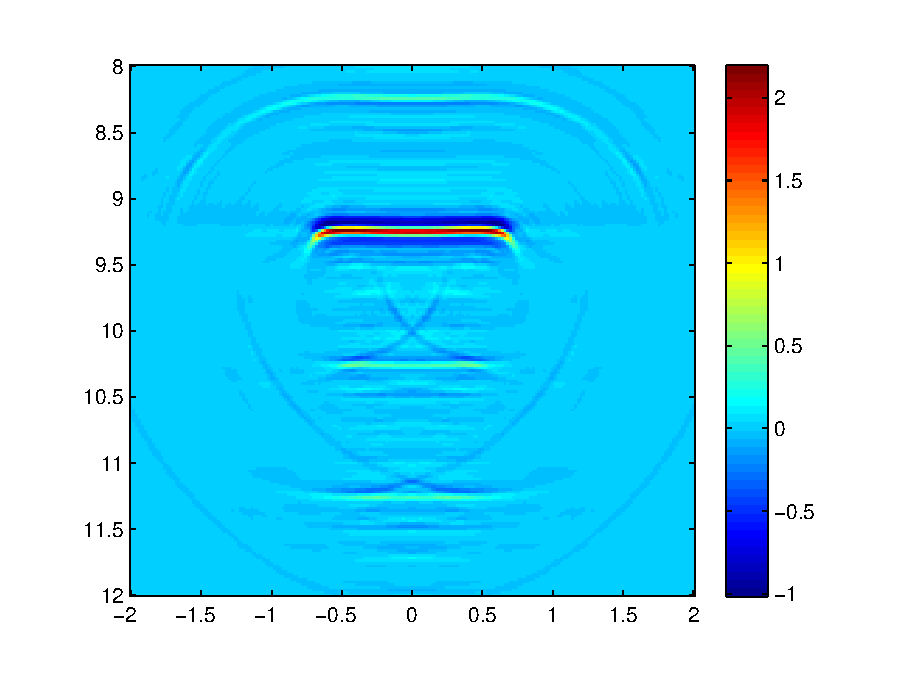
\includegraphics[width=0.32\textwidth]{./graphic/rectangle.eps}
\caption{Example 3: Imaging results of clamped obstacles
		with different shapes from top to below. The left row is imaged with single frequency data where $\om=3\pi$, The middle row is imaged with single frequency data where $\om=5\pi$ and The left row is imaged with multi frequency data}
\end{figure}
\end{frame}


\begin{frame}
\frametitle{Numerical Test: Two Obstacles}
\begin{figure}[h]
	
	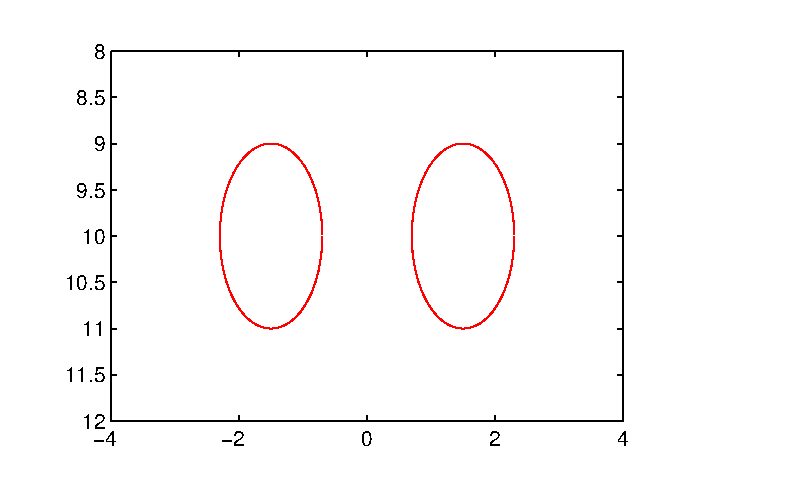
\includegraphics[width=0.32\textwidth,height=0.31\textheight]{./graphic/bi_circle_profile.eps}
	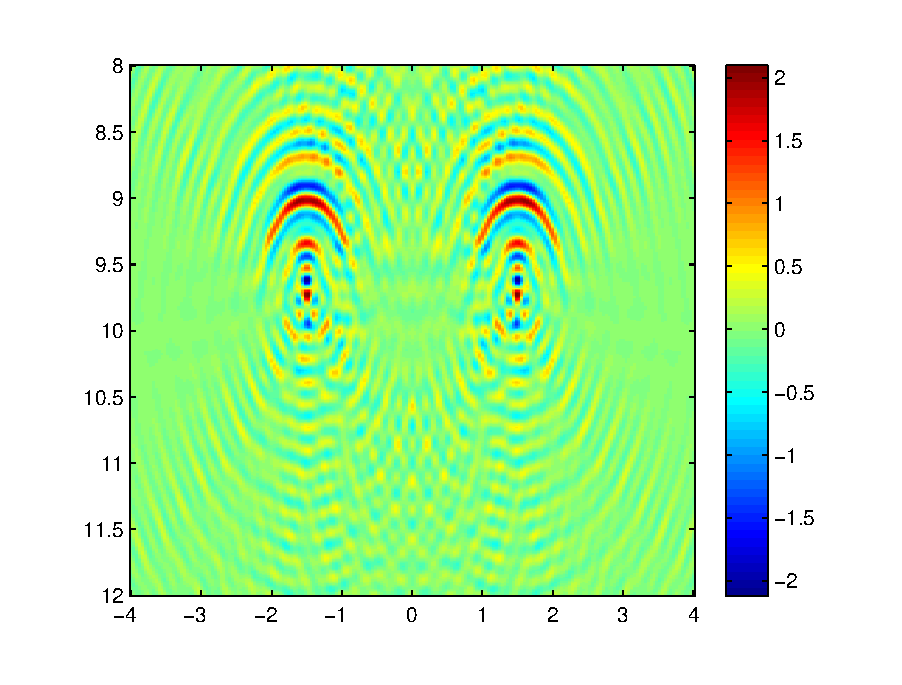
\includegraphics[width=0.32\textwidth]{./graphic/bi_circle_3pi.eps}
	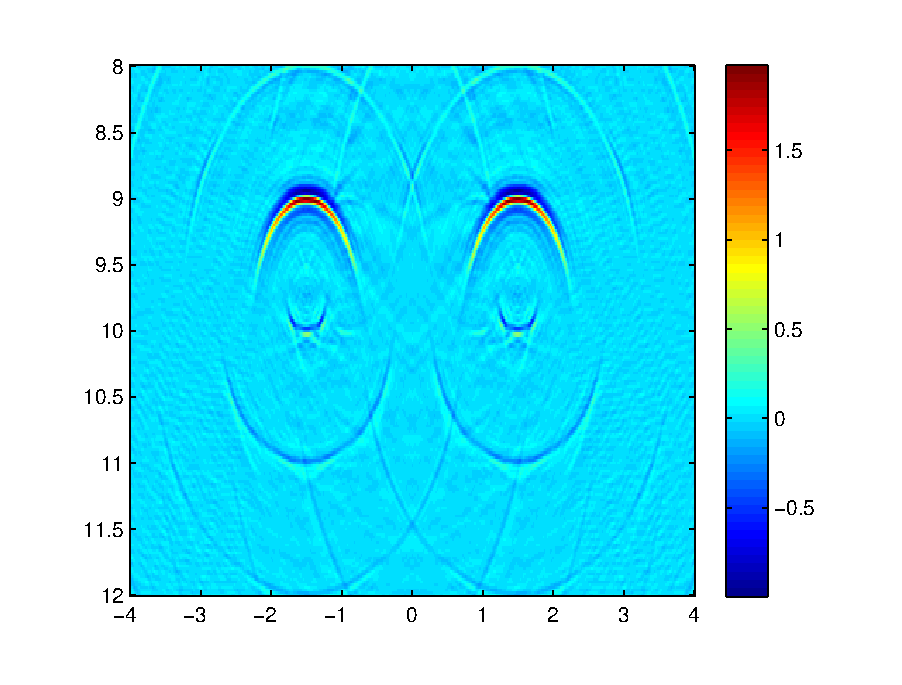
\includegraphics[width=0.32\textwidth]{./graphic/bi_circle.eps}\\
	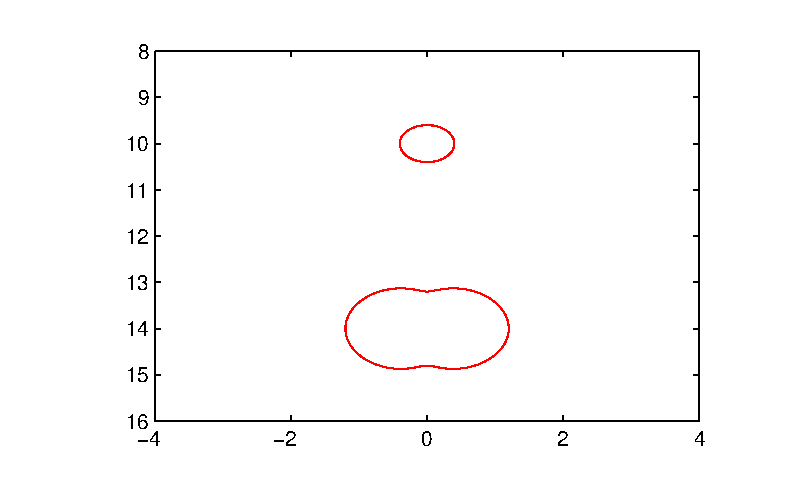
\includegraphics[width=0.32\textwidth,height=0.31\textheight]{./graphic/circle_0_4_peanut_1_profile.eps}
	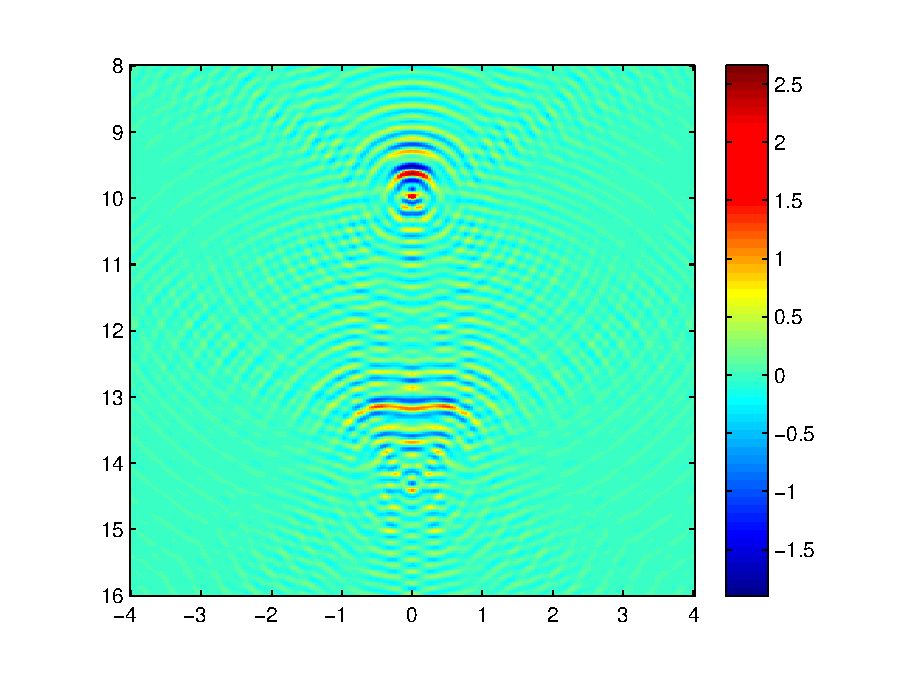
\includegraphics[width=0.32\textwidth]{./graphic/circle_0_4_peanut_1_3pi_1.eps}
	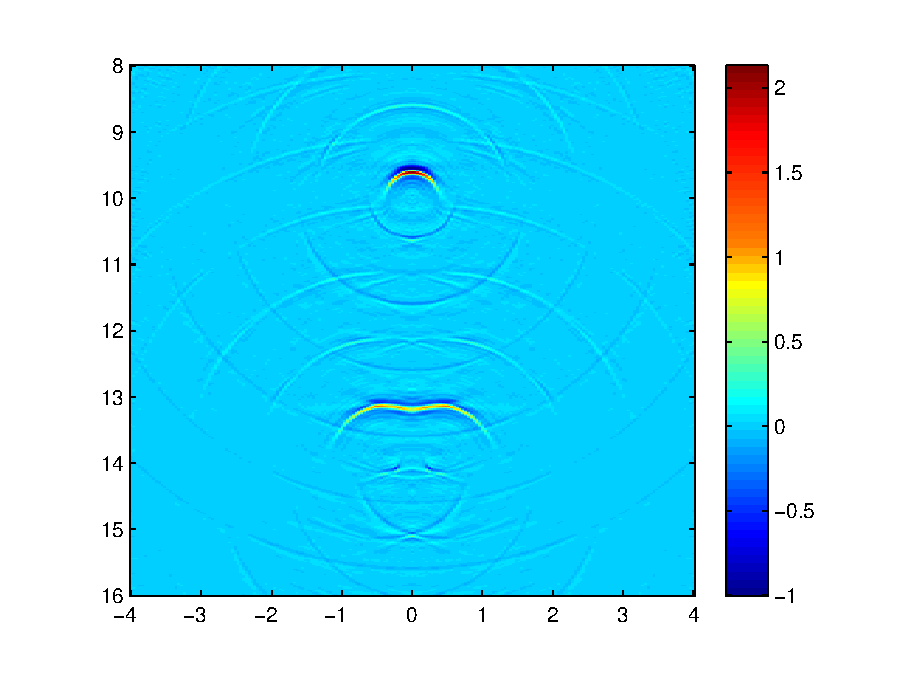
\includegraphics[width=0.32\textwidth]{./graphic/circle_0_4_peanut_1_multi_1.eps}
	
	\caption{Example 4:From left to right,  true obstacle model with two circles. the imaging result
		with single frequency data where $\om=3\pi$, the imaging result with multiple frequency data.}
\end{figure}
\end{frame}

\begin{frame}
\frametitle{Numerical Test: additive Gaussian noise}
\begin{figure}[h]
	\centering
	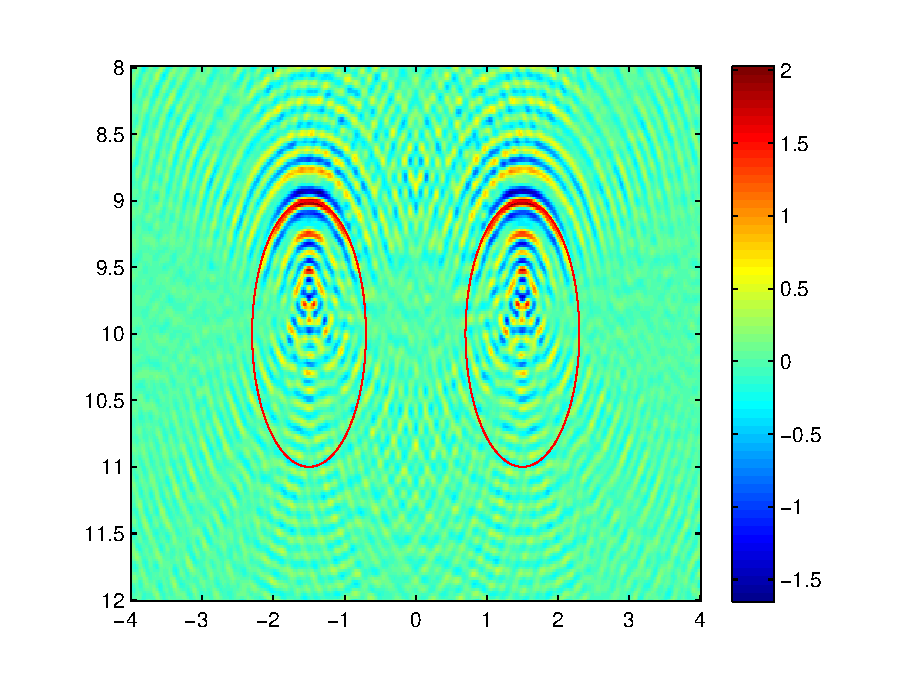
\includegraphics[width=0.32\textwidth]{./graphic/bi_circle_4pi_error2.eps}
	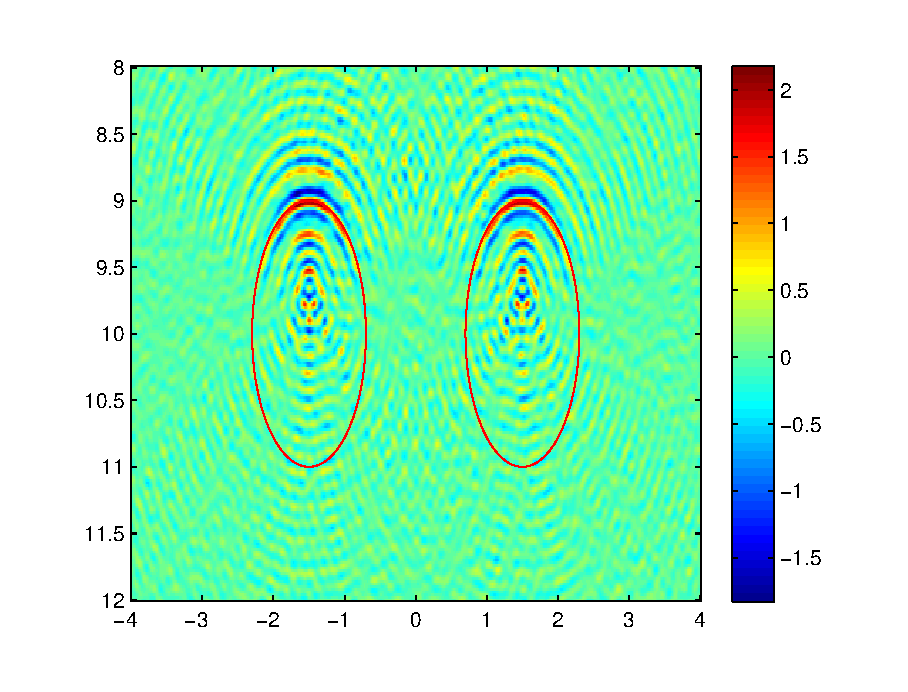
\includegraphics[width=0.32\textwidth]{./graphic/bi_circle_4pi_error4.eps}
	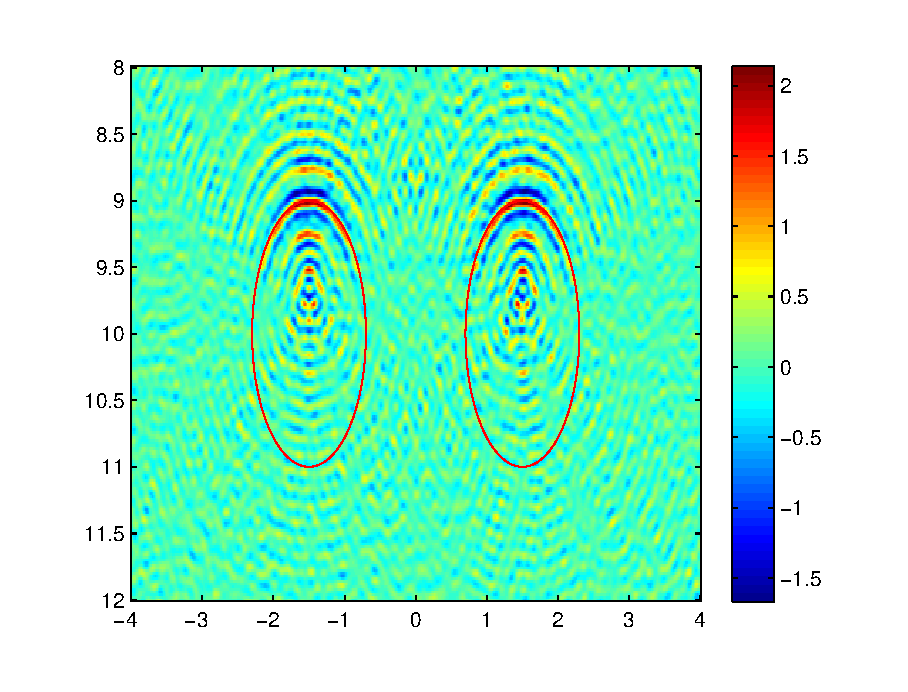
\includegraphics[width=0.32\textwidth]{./graphic/bi_circle_4pi_error6.eps}\\
	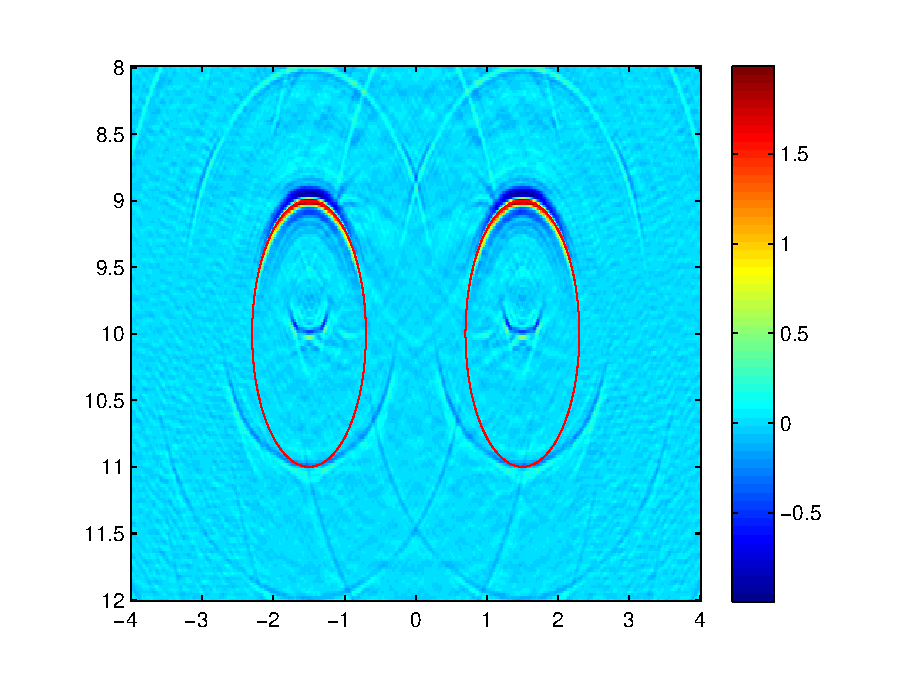
\includegraphics[width=0.32\textwidth]{./graphic/bi_circle_multi_2_8_error2.eps}
	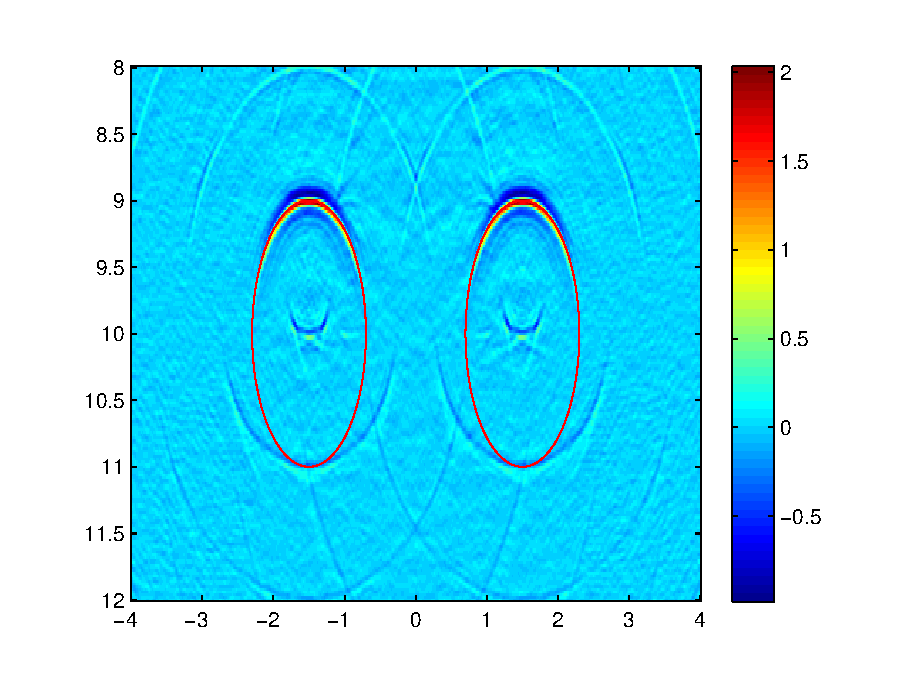
\includegraphics[width=0.32\textwidth]{./graphic/bi_circle_multi_2_8_error4.eps}
	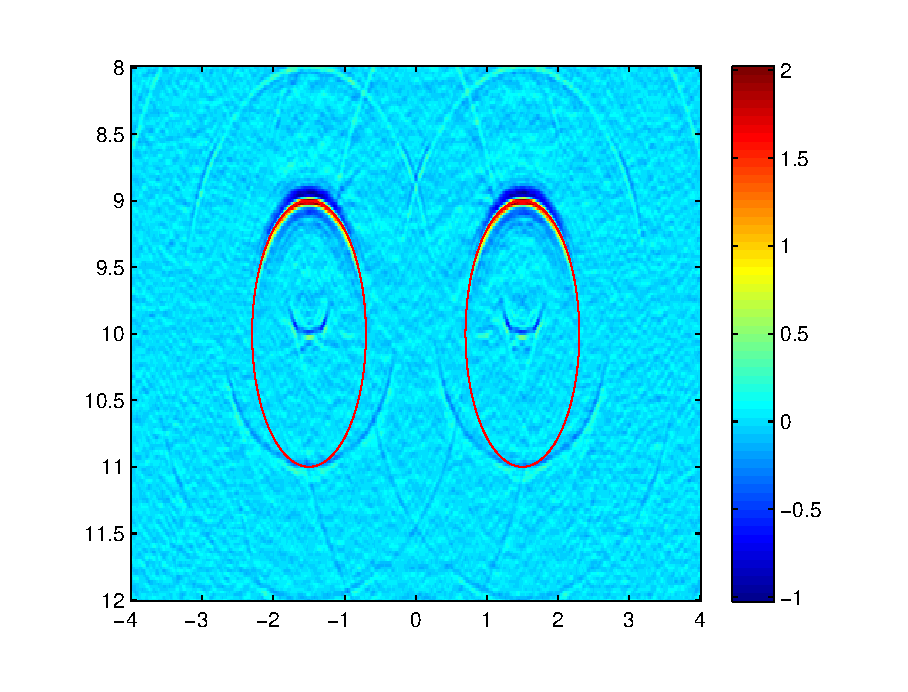
\includegraphics[width=0.32\textwidth]{./graphic/bi_circle_multi_2_8_error6.eps}
	
	\caption{Example 5: Imaging results of a clamped obstacle with noise levels $\mu =  0.2; 0.3; 0.4$ (from left to
		right). The top row is imaged with single frequency data where $\om=4\pi$, and the
		bottom row is imaged with multi-frequency data.}
\end{figure}
\end{frame}

\begin{frame}
\frametitle{Physical interpretation: high frequence}
Let y(s) be the arc length parametrization of the boundry $\Ga_D$ and $y_{\pm}(\eta_\theta)=y(s_{\pm})$ be the pionts such that $\nu(y(s_{\pm}))=\pm\eta_\theta$ and $\eta(y)$ be Gauss curvature. In the case of $\omega\gg1$, by stationary phase theorem and Kirchhoff approximation, the imaging function for the clamped obstacle is
\ben
\hat{I}_d(z)&\approx&\sqrt{8\pi k_p}\Im\mathbf{tr} \int_{0}^{\pi}((\lambda+2\mu)A_p(\theta)\eta_\theta e^{\i k_p (y_-(\eta_\theta)-z)\cdot \eta_\theta-\i\frac{\pi}{4}})^T\frac{\overline{F(z,y_-(\eta_\theta))}}{\sqrt{\vartheta(y_-(\eta_\theta))}}d\theta \\
&+&\sqrt{8\pi k_s}\Im\mathbf{tr} \int_{0}^{\pi}(\mu A_s(\theta)\eta_\theta^\perp e^{\i k_s (y_-(\eta_\theta)-z)\cdot \eta_\theta-\i\frac{\pi}{4}})^T\frac{\overline{F(z,y_-(\eta_\theta))}}{\sqrt{\vartheta(y_-(\eta_\theta))}}d\theta
\een
Now for z in the part of $\Ga_D$ which is back to $\Ga_0$, ie $\nu(z)\cdot\eta_\theta>0$ for any $\theta\in[0,\pi]$, we know that z and $y_{-}(\eta_\theta)$ are far away and thus $\hat{I}_d(z)\approx0$. By above formula , we can explain that one cannot image the back part of the obstacle with only the data collected on $\Ga_0$. This confirmed in our numerical examples.
\end{frame}


\begin{frame}
Our work:
\begin{itemize}
\item New form and asymptotic analysis of Green tensor in the half space..
\item Regularity estimate of direction elastic wave equation in the Half-space.
\item Mathematics analysis of point spread function.
\item Resolution analysis of Reverse Time Migration without any geometric optics approximation .
\item Scattered wave data simulation and numerical test of RTM.
\end{itemize}
Publication:
\begin{itemize}
\item Chen Z, Zhou S. {\it A Direct Imaging Method for Half-space Inverse Elastic Scattering Problems.} accepted.
\item Chen Z, Zhou S. {\it A Direct Imaging Method for Half-space Inverse Elastic Scattering Problems with Phaseless Data.} Preprint.
\item Chen Z, Zhou S. {\it Absense of Positive Eigenvalues for the Linearized Elasticity System in the Half
	Space} Preprint
\end{itemize}
\vspace{1cm}
\begin{flushright}
  \LARGE \textcolor[rgb]{1.00,0.00,0.00}{Thank you !}
\end{flushright}
\end{frame}

\begin{frame}
\frametitle{Future Plan}
\begin{itemize}
\item Direct and inverse elastic obstacle scattering problem in Muti-layers space or Half-space.
\item RTM for inverse rough surface problems using elastic waves.
\item RTM for invese scattering problems with phaseless data.
\end{itemize}
\end{frame}
%\end{CJK*}

\bibliography{./Thesis_Report}%
\end{document}

